\documentclass{report}
\usepackage[utf8]{inputenc}
\usepackage{amsmath}
\usepackage{ amssymb }
\usepackage{amsthm}
\usepackage[english]{babel}
\usepackage{listings}
\usepackage{ upgreek }
\usepackage[T1]{fontenc}
\usepackage[linguistics]{forest}
\usepackage{minted}
\usepackage{circuitikz}

%%%%%%%%%%%%%%%%%%%%%%%%%%%%%%%

%%%%%%%%%%%%%%%%%%%%%%%%%%%%%%%
\usepackage{hyperref}

\hypersetup{
    colorlinks=true,
    linkcolor=black,
    filecolor=black,      
    urlcolor=blue,
    pdftitle={Automata Theory},
    bookmarks=true,
    pdfpagemode=FullScreen,
    }
%%%%%%%%%%%%%%%%%%%%%%%%%%%%%%%%
\usepackage{natbib}
\usepackage{url}
\usepackage{parskip}
\usepackage{fancyhdr}
\usepackage{vmargin}

\title{Automata Theory}
\author{Liza Dahiya}
\date{}

\makeatletter
\let\thetitle\@title
\let\theauthor\@author
\let\thedate\@date
\makeatother

\pagestyle{fancy}
\fancyhf{}
\rhead{\theauthor}
\lhead{\thetitle}
\cfoot{\thepage}
%%%%%%%%%%%%%%%%%%%%%%%%%%%%%%%%%

\usepackage{tipa}
\usepackage{verbatim}
\usepackage{smartdiagram}

\newtheorem{theorem}{Theorem}
\newtheorem{corollary}{Corollary}[theorem]
\newtheorem{definition}{Definition}[chapter]
\newtheorem{proposition}{Proposition}[section]
%%%%%%%%%%%%%%%%%%%%%%%%%%%%%%%%%%%%%%%%%%%%%%%
\usepackage{tikz}
\usetikzlibrary{matrix,calc}

%isolated term
%#1 - Optional. Space between node and grouping line. Default=0
%#2 - node
%#3 - filling color
\newcommand{\implicantsol}[3][0]{
    \draw[rounded corners=3pt, fill=#3, opacity=0.3] ($(#2.north west)+(135:#1)$) rectangle ($(#2.south east)+(-45:#1)$);
    }


%internal group
%#1 - Optional. Space between node and grouping line. Default=0
%#2 - top left node
%#3 - bottom right node
%#4 - filling color
\newcommand{\implicant}[4][0]{
    \draw[rounded corners=3pt, fill=#4, opacity=0.3] ($(#2.north west)+(135:#1)$) rectangle ($(#3.south east)+(-45:#1)$);
    }

%group lateral borders
%#1 - Optional. Space between node and grouping line. Default=0
%#2 - top left node
%#3 - bottom right node
%#4 - filling color
\newcommand{\implicantcostats}[4][0]{
    \draw[rounded corners=3pt, fill=#4, opacity=0.3] ($(rf.east |- #2.north)+(90:#1)$)-| ($(#2.east)+(0:#1)$) |- ($(rf.east |- #3.south)+(-90:#1)$);
    \draw[rounded corners=3pt, fill=#4, opacity=0.3] ($(cf.west |- #2.north)+(90:#1)$) -| ($(#3.west)+(180:#1)$) |- ($(cf.west |- #3.south)+(-90:#1)$);
}

%group top-bottom borders
%#1 - Optional. Space between node and grouping line. Default=0
%#2 - top left node
%#3 - bottom right node
%#4 - filling color
\newcommand{\implicantdaltbaix}[4][0]{
    \draw[rounded corners=3pt, fill=#4, opacity=0.3] ($(cf.south -| #2.west)+(180:#1)$) |- ($(#2.south)+(-90:#1)$) -| ($(cf.south -| #3.east)+(0:#1)$);
    \draw[rounded corners=3pt, fill=#4, opacity=0.3] ($(rf.north -| #2.west)+(180:#1)$) |- ($(#3.north)+(90:#1)$) -| ($(rf.north -| #3.east)+(0:#1)$);
}

%group corners
%#1 - Optional. Space between node and grouping line. Default=0
%#2 - filling color
\newcommand{\implicantcantons}[2][0]{
    \draw[rounded corners=3pt, opacity=.3] ($(rf.east |- 0.south)+(-90:#1)$) -| ($(0.east |- cf.south)+(0:#1)$);
    \draw[rounded corners=3pt, opacity=.3] ($(rf.east |- 8.north)+(90:#1)$) -| ($(8.east |- rf.north)+(0:#1)$);
    \draw[rounded corners=3pt, opacity=.3] ($(cf.west |- 2.south)+(-90:#1)$) -| ($(2.west |- cf.south)+(180:#1)$);
    \draw[rounded corners=3pt, opacity=.3] ($(cf.west |- 10.north)+(90:#1)$) -| ($(10.west |- rf.north)+(180:#1)$);
    \fill[rounded corners=3pt, fill=#2, opacity=.3] ($(rf.east |- 0.south)+(-90:#1)$) -|  ($(0.east |- cf.south)+(0:#1)$) [sharp corners] ($(rf.east |- 0.south)+(-90:#1)$) |-  ($(0.east |- cf.south)+(0:#1)$) ;
    \fill[rounded corners=3pt, fill=#2, opacity=.3] ($(rf.east |- 8.north)+(90:#1)$) -| ($(8.east |- rf.north)+(0:#1)$) [sharp corners] ($(rf.east |- 8.north)+(90:#1)$) |- ($(8.east |- rf.north)+(0:#1)$) ;
    \fill[rounded corners=3pt, fill=#2, opacity=.3] ($(cf.west |- 2.south)+(-90:#1)$) -| ($(2.west |- cf.south)+(180:#1)$) [sharp corners]($(cf.west |- 2.south)+(-90:#1)$) |- ($(2.west |- cf.south)+(180:#1)$) ;
    \fill[rounded corners=3pt, fill=#2, opacity=.3] ($(cf.west |- 10.north)+(90:#1)$) -| ($(10.west |- rf.north)+(180:#1)$) [sharp corners] ($(cf.west |- 10.north)+(90:#1)$) |- ($(10.west |- rf.north)+(180:#1)$) ;
}

%Empty Karnaugh map 4x4
\newenvironment{Karnaugh}%
{
\begin{tikzpicture}[baseline=(current bounding box.north),scale=0.8]
\draw (0,0) grid (4,4);
\draw (0,4) -- node [pos=0.7,above right,anchor=south west] {cd} node [pos=0.7,below left,anchor=north east] {ab} ++(135:1);
%
\matrix (mapa) [matrix of nodes,
        column sep={0.8cm,between origins},
        row sep={0.8cm,between origins},
        every node/.style={minimum size=0.3mm},
        anchor=8.center,
        ampersand replacement=\&] at (0.5,0.5)
{
                       \& |(c00)| 00         \& |(c01)| 01         \& |(c11)| 11         \& |(c10)| 10         \& |(cf)| \phantom{00} \\
|(r00)| 00             \& |(0)|  \phantom{0} \& |(1)|  \phantom{0} \& |(3)|  \phantom{0} \& |(2)|  \phantom{0} \&                     \\
|(r01)| 01             \& |(4)|  \phantom{0} \& |(5)|  \phantom{0} \& |(7)|  \phantom{0} \& |(6)|  \phantom{0} \&                     \\
|(r11)| 11             \& |(12)| \phantom{0} \& |(13)| \phantom{0} \& |(15)| \phantom{0} \& |(14)| \phantom{0} \&                     \\
|(r10)| 10             \& |(8)|  \phantom{0} \& |(9)|  \phantom{0} \& |(11)| \phantom{0} \& |(10)| \phantom{0} \&                     \\
|(rf) | \phantom{00}   \&                    \&                    \&                    \&                    \&                     \\
};
}%
{
\end{tikzpicture}
}

%Empty Karnaugh map 2x4
\newenvironment{Karnaughvuit}%
{
\begin{tikzpicture}[baseline=(current bounding box.north),scale=0.8]
\draw (0,0) grid (4,2);
\draw (0,2) -- node [pos=0.7,above right,anchor=south west] {bc} node [pos=0.7,below left,anchor=north east] {a} ++(135:1);
%
\matrix (mapa) [matrix of nodes,
        column sep={0.8cm,between origins},
        row sep={0.8cm,between origins},
        every node/.style={minimum size=0.3mm},
        anchor=4.center,
        ampersand replacement=\&] at (0.5,0.5)
{
                      \& |(c00)| 00         \& |(c01)| 01         \& |(c11)| 11         \& |(c10)| 10         \& |(cf)| \phantom{00} \\
|(r00)| 0             \& |(0)|  \phantom{0} \& |(1)|  \phantom{0} \& |(3)|  \phantom{0} \& |(2)|  \phantom{0} \&                     \\
|(r01)| 1             \& |(4)|  \phantom{0} \& |(5)|  \phantom{0} \& |(7)|  \phantom{0} \& |(6)|  \phantom{0} \&                     \\
|(rf) | \phantom{00}  \&                    \&                    \&                    \&                    \&                     \\
};
}%
{
\end{tikzpicture}
}

%Empty Karnaugh map 2x2
\newenvironment{Karnaughquatre}%
{
\begin{tikzpicture}[baseline=(current bounding box.north),scale=0.8]
\draw (0,0) grid (2,2);
\draw (0,2) -- node [pos=0.7,above right,anchor=south west] {b} node [pos=0.7,below left,anchor=north east] {a} ++(135:1);
%
\matrix (mapa) [matrix of nodes,
        column sep={0.8cm,between origins},
        row sep={0.8cm,between origins},
        every node/.style={minimum size=0.3mm},
        anchor=2.center,
        ampersand replacement=\&] at (0.5,0.5)
{
          \& |(c00)| 0          \& |(c01)| 1  \\
|(r00)| 0 \& |(0)|  \phantom{0} \& |(1)|  \phantom{0} \\
|(r01)| 1 \& |(2)|  \phantom{0} \& |(3)|  \phantom{0} \\
};
}%
{
\end{tikzpicture}
}

%Defines 8 or 16 values (0,1,X)
\newcommand{\contingut}[1]{%
\foreach \x [count=\xi from 0]  in {#1}
     \path (\xi) node {\x};
}

%Places 1 in listed positions
\newcommand{\minterms}[1]{%
    \foreach \x in {#1}
        \path (\x) node {1};
}

%Places 0 in listed positions
\newcommand{\maxterms}[1]{%
    \foreach \x in {#1}
        \path (\x) node {0};
}

%Places X in listed positions
\newcommand{\indeterminats}[1]{%
    \foreach \x in {#1}
        \path (\x) node {X};
}
%%%%%%%%%%%%%%%%%%%%%%%%%%%%%%%%%%%%%%%%%%%%%%%
%---------------------------------------------------------
\usepackage{tikz}
\usetikzlibrary{shapes.geometric, arrows}
\tikzstyle{startstop} = [rectangle, rounded corners, minimum width=3cm, minimum height=1cm,text centered, draw=blue, fill=white]
\tikzstyle{process} = [rectangle, minimum width=3cm, minimum height=1cm, draw=white, fill=white]
\tikzstyle{arrow} = [thick,->,>=stealth]
%----------------------------------------------------------
\lstset{
  basicstyle=\ttfamily,
  mathescape
}

\usepackage{tikz}
\usetikzlibrary{automata, positioning, arrows}

%----------------------------------------------------------
\usepackage{xcolor}
\usepackage{graphicx}

\definecolor{codegreen}{rgb}{0,0.6,0}
\definecolor{codegray}{rgb}{0.5,0.5,0.5}
\definecolor{codepurple}{rgb}{0.58,0,0.82}
\definecolor{backcolour}{rgb}{0.95,0.95,0.92}

\lstdefinestyle{mystyle}{
    backgroundcolor=\color{backcolour},   
    commentstyle=\color{codegreen},
    keywordstyle=\color{magenta},
    numberstyle=\tiny\color{codegray},
    stringstyle=\color{codepurple},
    basicstyle=\ttfamily\footnotesize,
    breakatwhitespace=false,         
    breaklines=true,                 
    captionpos=b,                    
    keepspaces=true,                 
    numbers=left,                    
    numbersep=5pt,                  
    showspaces=false,                
    showstringspaces=false,
    showtabs=false,                  
    tabsize=2
}
\lstset{style=mystyle}
%----------------------------------------------------------
%----------------------------------------------------------

%----------------------------------------------------------
%----------------------------------------------------------

\setcounter{tocdepth}{1}

\begin{document}
\begin{titlepage}
	\centering
    \vspace*{0.5 cm}
    \textsc{\LARGE Indian Institute of Technology Bombay}\\[2.0 cm]
        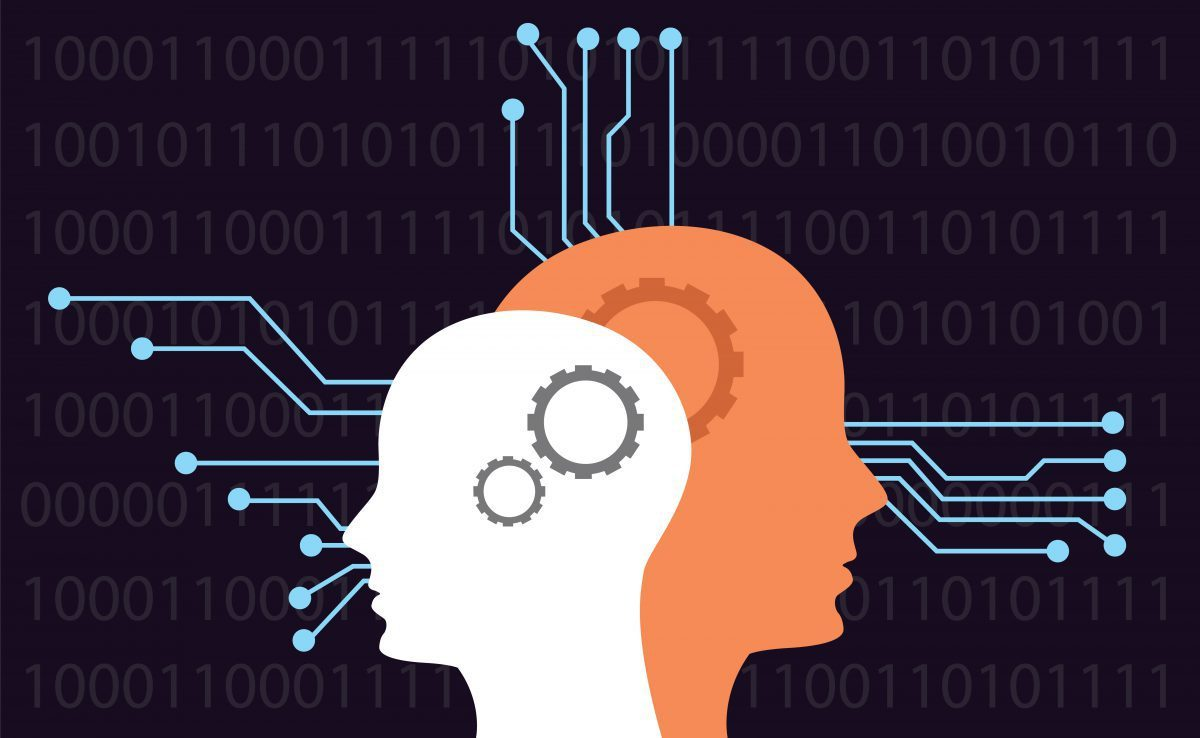
\includegraphics[scale = 0.25]{cover.jpg}\\[1.0 cm]	
        
	\rule{\linewidth}{0.2 mm} \\[0.4 cm]
	{ \huge \bfseries \thetitle}\\
	\rule{\linewidth}{0.2 mm} \\[1.5 cm]
	
	\begin{minipage}{0.4\textwidth}
			\begin{center} \large
			\textbf{Liza Dahiya}\\ 
			\textbf{Roll No.:} 190050063\\
			Computer Science \& Engineering\\
            \textbf{Mentor:} Shrey Singhai\\
		\end{center}
        
	\end{minipage}\\[2 cm]

\end{titlepage}

\tableofcontents
\newpage

\subsubsection{\Large{
\begin{center}
    Brief Introduction
\end{center}  }}
I, Liza Dahiya, began learning with the introduction of Propositional Logic and Natural Deduction since it is good to have a strong knowledge of logic in computer science before delving into the Automata theory.

After which I, formally begin with the Automata theory and describe the Finite Automaton. Various examples are included for understanding the different types of finite automaton. Then we deal with regular expressions which are used for describing regular languages for finite automaton. Then Context-Free Grammar and Pushdown Automaton are introduced which are another way for describing languages to broaden the spectrum of understanding the Automata Theory. 

Final chapters are dedicated for the understanding of digital circuits before trying to code those in Intel Quartus (in VHDL) for having a sense of practical application for the theory. 

\chapter{Propositional Logic}
\section{Introduction}
\textbf{Declarative Sentences} or \textit{propositions} are the ones which in principle can be argued as being true or false. Propositional Logic deals with such propositions. \textbf{Examples:} \textbf{Goldbach's conjecture- }Every even natural number $>$ 2 is the sum of two prime numbers. \\
\\
\textbf{\large{Syntax}}
\begin{itemize}
    \item $\neg$ : Negation
    \item $\vee$ : At least one of p or q is true
    \item $\wedge$ : Both p and q are true
    \item $\to$ : If this, then this
\end{itemize}

\textbf{Binding Proprieties:} $\neg$ binds more tightly than $\vee$ or $\wedge$, which binds tighter than $\to$. In the absence of parentheses, $p \to q \vee r$ is read as $p \to (q \vee r$).  

%-----NATURAL DEDUCTION-------
%-----------------------------

\section{Natural Deduction}
Natural deduction allows us to infer \textit{conclusions} from some formulae called as \textit{premise}. The following expression is called as \textit{sequent}:
\vspace{-1.5em}
\begin{center}
$$\phi_1, \phi_2,\ldots, \phi_n \vdash \psi$$
\end{center} 

    \subsection{Rules of Natural Deduction}
    Rules of natural deduction allows us to conclude various formulas from some given formulas and hence provide proof for a sequent:
    \par
    %---------CONJUGATION------------
    \begin{itemize}
        \item \textbf{Rule for Conjugation:} 
            \begin{itemize}
                \item {\textbf{Rule for and-introduction:}} It allows us to conclude $\phi$ $\wedge$ $\psi$, given that $\phi$ and $\psi$ are concluded separately:
                \begin{center}
                 $\dfrac{\phi \hspace{0.2cm} \psi}{\phi \wedge \psi}$ $\wedge i$
                \end{center}
             
                \item \textbf{Rules for and-elimination:} If you have a proof of  $\phi \wedge \psi$ then, $\wedge e_1$ rule allows you to get a proof of $\phi$:\\
                \begin{center}
                    $\dfrac{\phi \wedge \psi}{\phi}$   $\wedge e_1$ \hspace{2cm}
                    $\dfrac{\phi \wedge \psi}{\psi}$   $\wedge e_2$
                \end{center}
            \end{itemize}
        
    %-------DOUBLE NEGATION---------
        \item{\textbf{Rules for Double Negation}} Intuitively, $\neg \neg \phi$ expresses same meaning as $\phi$ does. The following are rules for introduction \& elimination respectively.
            \begin{itemize}
               \item \textbf{Introduction: }\hspace{0.2cm} $\dfrac{\phi}{\neg \neg \phi}$\hspace{0.2cm} $\neg \neg i$
               
               \item \textbf{Elimination: } \hspace{0.2cm} $\dfrac{\neg \neg \phi}{\phi}$ \hspace{0.2cm} $\neg \neg e$
            \end{itemize}
    
     %-------MODULUS PONENS---------
        \item{\textbf{Modulus Ponens:}}is the rule for eliminating-implication, popularly known as its Latin name, \textit{Modulus Ponens}.
        \begin{center}
            $\dfrac{\phi \hspace{0.2cm} \phi \to \psi}{\psi}$ $\to e$
        \end{center}
        
    %-------MODULUS TONEUS---------
        \item{\textbf{Modulus Toneus:}} This rule is derived from other rules.
        \begin{center}
            $\dfrac{\phi \to \psi \hspace{0.2cm} \neg \psi}{\neg \phi}$ $MT$
        \end{center}
        
    %-------INTRODUCTION IMPLICATION---------
        \item\textbf{{Introduction implication:}} In this rule, we open a box by assuming $\phi$, and then applying laws of natural deduction, we derive $\psi$. Finally, when we close a box, we have $\phi \to \psi$.
        \\
    %     \begin{center}
	   % $\boxed {{\phi} \\ \vdots \\ \psi}$
    %     \end{center}
    
    \[ \frac{
      \boxed{
        \begin{array}{c}
          \phi\\
          \vdots\\
          \psi
        \end{array}
      }
    }{
      \phi \rightarrow \psi
    }
    \rightarrow i
\]
\\
    
    %-------DISJUNCTION---------
        \item{\textbf{Rules for Disjunction}}
         \begin{itemize}
             \item \textbf{Introduction:} We may conclude $\phi \vee \psi$ given either of $\phi$ or $\psi$ is concluded before:
             \begin{center}
                    $\dfrac{\phi}{\phi  \vee \psi}$   $\vee i_1$ \hspace{2cm}
                    $\dfrac{\psi}{\phi \vee \psi}$   $\vee i_2$
                \end{center}
             \item \textbf{Elimination:}  The following steps need to be followed while implementing elimination rule for disjunction:
             \begin{itemize}
                 \item First, we assume $\phi$ is true and have to come up with a proof of $\chi$.
                 \item Next, we assume $\psi$ is true and need to give a proof of $\chi$ as well. 
                 \item Given these two proofs, we can infer $\chi$ from the truth of $\phi \vee \psi$, since our case analysis above is exhaustive. \\
             \end{itemize}
             These steps are summarised in the formula below: \\
             \begin{center}
                 $\dfrac{\phi \vee \psi \hspace{0.2cm} \boxed{
        \begin{array}{c}
          \phi\\
          \vdots\\
          \chi
        \end{array}
      } \hspace{0.2cm} \boxed {
      \begin{array}{c}
          \psi\\
          \vdots\\
          \chi
        \end{array}
      }}{\chi}$ $\vee e$
             \end{center}
         \end{itemize}
        
    %-------NEGATION---------
        \item{\textbf{Negation}}
            \begin{itemize}
                \item \textbf{Bottom Elimination:} The fact that $\bot$ can prove anything is encoded in our calculus by the proof rule bottom-elimination:
                    \begin{center}
                        $\dfrac{\bot}{\phi}$ $\bot e$
                    \end{center}
                \item \textbf{Not- Elimination:} The fact that $\bot$ itself represents a contradiction is encoded by the proof rule not-elimination: 
                     \begin{center}
                         $\dfrac{\phi \hspace{0.2cm} \neg \phi}{\bot}$ $\neg e$
                     \end{center}
            \end{itemize}
\end{itemize}

\subsection{Proof by Contradiction}
If we assume $\neg \phi$ (while opening a box) and then obtain $\bot$ i.e. contradiction in the box, we are entitled to deduce $\phi$. \\
\par

\subsection{Law of Excluded Middle (LEM)}
The law just says that $\phi \vee \neg \phi$ is true whatever $\phi$ is, true or false. 
\begin{center}
    $\dfrac{ }{\phi \vee \neg \phi}$ $LEM$
\end{center}


\section{Semantics}
\begin{definition}{}
A \textit{valuation} of a formula $\phi$ is an assignment of each propositional atom in $\phi$ to a truth value (i.e. True or False).
\end{definition}
$\phi_1, \phi_2,\ldots, \phi_n \vDash \psi$ iff whenever $\phi_1, \phi_2,\ldots, \phi_n$ evaluates to T (true) so does $\psi$. $\vDash$ is called \textbf{semantics entails}. 

\subsection{Soundness of Propositional Logic}
\begin{theorem}
Let $\phi_1, \phi_2,\ldots, \phi_n, \psi$ be propositional logic formulas. If $\phi_1, \phi_2,\ldots, \phi_n \vdash \psi$ is valid, then $\phi_1, \phi_2,\ldots, \phi_n \vDash \psi$ holds. 
\end{theorem}
%include screenshots of proof sections

\subsection{Completeness of Propositional Logic}
\begin{theorem}
If $\phi_1, \phi_2,\ldots, \phi_n \vdash \psi$ is, then there exists a natural deduction proof for the sequent $\phi_1, \phi_2,\ldots, \phi_n \vDash \psi$ holds. 
\end{theorem}
In the process of proving completeness of propositional logic, we use definitions and theorems, which are stated below:
\begin{definition}{}
A formula of propositional logic $\phi$ is called a tautology, iff it evaluates T under all its valuations, i.e. iff $\vDash \phi$  
\end{definition}

\begin{theorem}
If $\vDash \eta$ holds, then $\vdash \eta$ is valid. In other words, if $\eta$ is valid, then $\eta$ is theorem.
\end{theorem}

\subsection{Combining soundness and completeness}
Let $\phi_1, \phi_2,\ldots, \phi_n, \psi$ be propositional logic formulas. This $\phi_1, \phi_2,\ldots, \phi_n \vdash \psi$ hols \textbf{iff} $\phi_1, \phi_2,\ldots, \phi_n \vDash \psi$ holds. 
%include screenshots of proof sections
\section{Normal Forms}
\begin{definition}
    $\phi$ and $\psi$ are two propositional logic. We say that $\phi$ and $\psi$ are semantically equivalent iff $\phi \vDash \psi$ and $\psi \vDash \phi$.
    We write this as $\phi \equiv \psi$
\end{definition}

\begin{definition}
    A \textbf{literal} $L$ is either an atom $p$ or the negation of an atom $\neg p$.
    A formula \textbf{$C$} is in \textbf{conjunctive normal form (CNF)} if it is a conjugation of clauses, where each clauses \textbf{$D$} is \textbf{disjunction} of literals.\\
    \begin{center}
        $L ::= p|\neg p$\\
        $D ::= L|L \vee D$\\
        $C ::= D|D \wedge C$
    \end{center}
    \end{definition}
\textbf{Examples:}
\begin{itemize}
    \item $(\neg q \vee p \vee r) \wedge (\neg p \vee r) \wedge q$: This is in CNF.
    \item $(\neg (q \vee p) \vee r) \wedge (q \vee r)$: This is not in CNF.
\end{itemize}
\begin{proposition}
    Let $\phi$ be a formula of propositional logic. Then $\phi$ is satisfiable i.e. there is a valuation where $\phi$ evaluates to T, iff $\neg \phi$ is not valid. 
\end{proposition}
%definitions, lemma, include programs
%screenshot of worked out examples
\subsection{The CNF Algorithm}
The CNF algorithm computes CNF as an output for a given input $\phi$. The following are the three requirements that CNF needs to satisfy:
\begin{enumerate}
    \item CNF terminates for all formulas of propositional logic as input;
    \item for each such input, CNF outputs an equivalent formula; and
    \item all output computed by CNF is in CNF.
\end{enumerate}
The algorithm involves three steps:
\subsubsection{IMP\_FREE($\phi)$}
First task is to remove all of the sub formulas in the form $\psi \to \eta$ by $\neg \psi \vee \eta$. This process has to be done recursively, for there might be implications in $\psi$ or $\eta$. Hence, finally the entire formula is made implication free.

\subsubsection{NNF(IMP\_FREE($\phi$))}
Negation Normal Forms (NNF) are the formulas which only \textit{negate} atoms. NNF is applied after making sure that the formula is implication free. Following is the code for applying NNF on a formula $\phi$: \\

\begin{lstlisting}[language=Python]
def function (NNF(($\phi$)):
    #precondition: $\phi$ is implication free
    #postcondition: NNF($\phi$) computes NNF of $\phi$
    begin function
    case 
    $\phi$ is literal: return $\phi$
    $\phi$ is $\neg \neg \phi_1$: return NNF($\phi_1$)
    $\phi$ is $\phi_1 \wedge \phi_2$: return NNF($\phi_1$) $\wedge$ NNF($\phi_2$)
    $\phi$ is $\phi_1 \vee \phi_2$: return NNF($\phi_1$) $\vee$ NNF($\phi_2$)
    $\phi$ is $\neg(\phi_1 \wedge \phi_2)$: return NNF($\neg \phi_1$) $\vee$ NNF($\neg \phi_2$)
    $\phi$ is $\neg(\phi_1 \vee \phi_2)$: return NNF($\neg \phi_1$) $\wedge$ NNF($\neg \phi_2$)
    end case
    end function
\end{lstlisting}
%might include worked out example
\par
After applying both of the above, we obtain NNF(IMPL\_FREE($\phi$)) $= \phi'$; and now $\phi' \equiv \phi$. We now apply CNF($\phi'$), which is discussed in the subsection below:
\subsubsection{CNF($\phi$)}
We begin by defining the function for computing CNF of $\phi$:\\
\begin{lstlisting}[language=Python]
def function CNF($\phi$):
    #precondition:$\phi$ is implication-free and in NNF
    #postcondition: CNF($\phi$) computes equivalent CNF for $\phi$
    begin function
    case
    $\phi$ is literal: return $\phi$
    $\phi$ is $\phi_1 \wedge \phi_2$: return CNF($\phi_1$) $\wedge$ CNF($\phi_2$)
    $\phi$ is $\phi_1 \vee \phi_2$: return DISTR(CNF($\phi_1$), CNF($\phi_2$))
    end case
    end function
\end{lstlisting}
Here in case 3, when $\phi$ is in the form of $\phi_1 \vee \phi_2$, if we call CNF recursively on $\phi_i$ to get $\eta_i$; but in this case we cannot return $\eta_1 \vee \eta_2$, since the formula will not be in CNF form and the 3rd requirement will not be fulfilled. \\
\par
Hence we introduce a new function DISTR($\eta_1$,$\eta_2$) which uses the distributivity of conjugations and disjunctions, and whose code is provided below: \\
\begin{lstlisting}[language=Python]
def function DISTR($\eta_1, \eta_2$):
    #precondition:$\eta_1, \eta_2$ are in CNF
    #postcondition: DISTR($\eta_1, \eta_2$) computes a CNF for $\eta_1 \vee \eta_2$
    begin function
    case
    $\eta_1$ is $\eta_{11} \wedge \eta_{12}$: return DISTR($\eta_{11}, \eta_2$) $\wedge$ DISTR($\eta_{12}, \eta_2$) 
    $\eta_2$ is $\eta_{21} \wedge \eta_{22}$: return DISTR($\eta_1, \eta_{21}$) $\wedge$ DISTR($\eta_1, \eta_{22}$) 
    otherwise: return $\eta_1 \vee \eta_2$
    end case
    end function
\end{lstlisting}

\section{Horn Formula}
\begin{definition}
    A \textbf{Horn formula} is a formula of $\phi$ of propositional logic if it can be generated as an instance of H in this grammar:
    \begin{center}
        $P::= \bot |  \top  | p$\\
        $A::= P| A \wedge P$\\
        $C::= A \to P$\\
        $H::= C| C \wedge H$
    \end{center}
\end{definition}
\textbf{Example:}\par
\begin{itemize}
    \item $(p \wedge q \wedge s \to p) \wedge (q \wedge r \to p) \wedge (p \wedge s \to s)$: This is a Horn Formula.
    \item $(p \wedge q \wedge s \to \bot) \wedge (\neg q \wedge r \to p) \wedge (\top \to s)$: This is not a Horn Formula, since $(\neg q \wedge r)$ is not a conjugation of atoms, $\top$ or $\bot$. 
\end{itemize}
\subsection{Satisfiability of Horn Formula}
The following algorithm is used to check satisfiability of a Horn Formula. 

\begin{lstlisting}[language=Python]
def function HORN($\phi$):
    #precondition:$\phi$ is a Horn formula
    #postcondition: HORN($\phi$) decides satisfiability of $\phi$
    begin function
    mark all occurances of $\top$ in $\phi$
    while there is a conjuct $P_1 \ldots P_{ki} \wedge P'$ of $\phi$ such that all $P_j$            are marked but $P'$ is not if mark $P'$
    end while
    if $\bot$ is marked then return 'unsatisfiable'
    else return 'satisfiable'
    end function
\end{lstlisting}

\begin{theorem}
The algorithm HORN is correct for the satisfiability decision problem of Horn formulas and has no more than n +1 cycles in its whilestatement if n is the number of atoms in $\phi$. In particular, HORN always terminates on correct input.
\end{theorem}
Hence, according to the above theorem this algorithm terminates on all Horn formulas $\phi$ as input and that its output (= its decision) is always correct. 

%theorem, program 
\section{Resolution}
Resolution is a technique used to check if a formula in CNF is satisfiable.\\
Let $C_1$ and $C_2$ are two clauses. Assume $A \in C_1$ and $\neg A \in C_2$. Then the clause:\\
\begin{center}
R=$(C_1-{A}) \cup (C_2-{\neg A})$ is a resolvent of $C_1$ and $C_2$. 
\end{center}
\subsection{3 Rules of Resolution}
\begin{enumerate}
    \item Let $G$ be any formula. Let $F$ be the CNF formula resulting from the CNF algorithm applied to $G$. Then $G \vdash F$.
    \item Let $F$ be a formula in CNF, and let $C$ be a clause in $F$. Then $F \vdash C$.
    \item Let $F$ be a formula in CNF. Let $R$ be a resolvent of two clauses of $F$. Then $F \vdash R$ 
\end{enumerate}
\subsection{Completeness}
There is an $m$ such that $Res^m (F)=Res^{m+1} (F)$, where $F$ is any formula in CNF. This is denoted by $Res^*(F)$.
\begin{theorem}
Let $\psi$ be any formula, convert it into CNF form, say $\zeta$, then $\phi$ is satisfiable \textbf{iff} $\emptyset \notin Res^*(F)$ . 
\end{theorem}

\chapter{Finite Automata}
\section{Introduction}
A finite automaton is a formal system that stores only finite amount of information. It can not be used when indefinite amount of data is required. Finite automaton can be used to tell whether two automaton perform the same task or not or whether there exists any smaller automaton that does the same thing. 
\begin{itemize}
    \item Information is stored in the form of \textit{\textbf{states}}, $Q$.
    \item State changes in response to \textit{\textbf{inputs}}.
    \item Rules that tell how the state changes in response to inputs are called \textit{\textbf{transitions}}, $\delta$. 
    \item In the automaton, we designate some special states to be \textit{\textbf{accepting states}}. If an input word moves forward the automaton to an accepting state, we say that it is \textit{\textbf{accepted}}. Otherwise, \textbf{\textit{rejected}}.
    \end{itemize}

    \subsection{Alphabets}
    \begin{itemize}
        \item The domain of strings is called \textit{\textbf{alphabet}} usually denoted by $\Upsigma$.
        \item The elements of alphabet are called as \textit{\textbf{letters}}.
        \item Inputs are sequences of letters, usually called \textit{words} (or string). \par
        $\Upsigma^0$ is a string of length 0. There is only one single empty string, denoted by $\epsilon$.
        $$\Upsigma^0 \triangleq {\epsilon}$$ 
        \item $\Upsigma^*$ is used to specify the union of all lengths of alphabets.
        $$\Upsigma^* \triangleq \Upsigma^1 \cup \Upsigma^2 \cup \Upsigma^3 \cup \ldots$$
        \item $\Upsigma^+$ doesn't contain the empty string.  
    \end{itemize}
    \subsection{Languages}
    The set of strings accepted by an automaton A is the \textbf{\textit{language}} of that automaton.
    Let $\Upsigma$ be an alphabet. Then a subset of $\Upsigma^*$ is called language. \textbf{Example:}
    \begin{enumerate}
        \item $L_{eq} = \{0^n1^n|n\geqslant0\}$
        \item $L_{prime}$ = {$w|w$ is binary encoding of a prime number}\\
              Consider a problem to check if a number n is a prime number?
              Let binary(n) be the binary encoding of n, then we need to check:
            $$binary(n) \in L_{prime}$$
    \end{enumerate}
    
\section{Deterministic Finite Automaton}
    The word deterministic means that there is a unique transition going on for every state and input symbol. A deterministic finite automaton(DFA) A is a five-tuple represented by:
    $$(Q,\delta,\Upsigma,q_0,F)$$
    where, \begin{itemize}
        \item $Q$ is a finite set of states.
        \item $\Upsigma$ is a finite set of input symbols.
        \item $\delta$ is a transition function.
        \item $q_0 \in Q$ is the start/initial state, and
        \item $F \subseteq Q$ is a set of accepting states.
    \end{itemize}
    \subsection{Transition Function}
    It takes up two inputs: a state and an input symbol and returns the next state.
    $\delta(q,a)$= the state that the DFA goes to when it is in state q and an input a is received.
    \begin{itemize}
        \item Note: always a next state – add a \textbf{dead state} if no transition.
    \end{itemize}
    \subsection{Graphs}
    DFA can be represented as graphs with nodes represented the states $q$ and the transition $\delta$ is represented by the loops. \\ \textbf{Example:}\par
    In the figure shown, state $q_1$ represent string that doesn't have any 11's and doesn't end in 1, while state $q_2$ represents string ending in 1 but with no consecutive 11's. And finally state $q_3$ represents string with consecutive 11's and hence a \textbf{dead state} since on any further input no transition can be made to any other state since we've already detected at least one pair of consecutive 11's. 
    \begin{figure}[ht] 
    \centering 
    \begin{tikzpicture}
        \node[state, accepting, initial] (q1) {$q_1$};
        \node[state, accepting, right of=q1, xshift=1cm] (q2) {$q_2$};
        \node[state, right of=q2, xshift=1cm] (q3) {$q_3$};
        \draw (q1) edge[loop below] node{0} (q1)
        (q1) edge[above] node{1} (q2)
        (q2) edge[above] node{1} (q3)
        (q2) edge[bend right, above] node{0} (q1)
        (q3) edge[loop above] node{0, 1} (q3);
    \end{tikzpicture}
    \caption{Strings ending with no 11's}
    \label{fig:my_label}
    \end{figure}

\subsection{Transition table}
The graph represented in the above section can also be presented as a transition table with rows represented states and columns represented input symbols and the final states being represented as $*$.

    \begin{center}
    \begin{tabular}{||c c c||} 
     \hline
      & 0 & 1 \\ [0.5ex] 
    \hline\hline
    $*$A & A & B \\ 
    \hline
    $*$B & A & C\\
    \hline
    C & C & C \\ [1ex]
    \hline
    \end{tabular}
    \end{center}
\subsection{Extending Transition Function}
Let $(Q,\delta,\Upsigma,q_0,F)$ be a DFA. An extended transition function also takes two arguments. The first argument is a state q and the second argument is a string w. It returns a state just like the transition function discussed in the previous sections. It can be defined as the state in which the FA ends up, if it begins in state q and receives string x of input symbols.  Let $\hat{\delta}: Q X \Upsigma^* \to Q$ be defined as follows:
    $$\hat{\delta} (q,\epsilon) \triangleq q$$
    $$\hat{\delta} (q,wa) \triangleq \delta (\hat{\delta} (q,wa),a)$$

\subsection{Regular languages}
    A language L is regular if it is the language accepted by some DFA. \\
   \textbf{Example of a Regular language}
    \begin{itemize}
        \item $L_2$ = $\{w|w$ in $\{0,1\}^*\}$ and w is viewed as binary integer is divisible by 23.
        \item $L_2$ = $\{w|w$ in $\{0,1\}^*\}$ and w is viewed as \textbf{reverse} of binary integer is divisible by 23.
    \end{itemize}
    \begin{theorem}
    The reverse of a regular language is also regular.
    \end{theorem}
   \textbf{Example of a Non-Regular language}
    \begin{itemize}
        \item $L_1 = \{0^n1^n|n\geqslant0\}$
        \item $L_2$ = $\{w|w$ in $\{(,)\}^*\}$ and w is \textbf{balanced}\par
        Balanced parentheses are those sequences of parentheses that can appear in an arithmetic expression. Ex: (),()(),(()), etc.
        \end{itemize}

\subsection{Worked Out Example}
    \par \textbf{Find a DFA for {$w|$ 01s occur somewhere}}.
    \begin{figure}[ht] 
    \centering 
    \begin{tikzpicture}
        \node[state, initial] (q0) {$q_0$};
        \node[state, right of=q0, xshift=1cm] (q1) {$q_1$};
        \node[state, below of=q1, yshift=-1cm] (q2) {$q_2$};
        \node[state, accepting, right of=q1, xshift=1cm] (q3) {$q_3$};
        \draw (q0) edge[above] node{0} (q1)
        (q0) edge[below, bend right] node{1} (q2)
        (q1) edge[loop above] node{0} (q1)
        (q1) edge[above] node{1} (q3)
        (q2) edge[loop below] node{1} (q2)
        (q2) edge[bend right, above] node{0} (q3)
        (q3) edge[loop above] node{0, 1} (q3);
    \end{tikzpicture}
    \caption{Strings with 01's somewhere}
    \label{fig:my_label}
    \end{figure}
    In the figure above, $q_0$ is the initial start state, the automaton moves to the state $q_1$ on receiving an input symbol 0 and to state $q_2$ on receiving an input symbol 1. We mark $q_3$ as the accepting state \& when $q_1$ will receive an input 1, it'll go to the final state $q_3$ as we can say that 01 was present somewhere in the string of input symbols. Other transitions can also be explained similarly.  


\section{Non-Deterministic Automaton}
A non-deterministic finite automaton has the ability to be in several states at once. Transitions from a state on an input symbol can be to any set of states. Start in one of the start state. Accept if any sequence of choices leads to a final state. The formal symbols used in NFA are quite similar to DFA with the only difference being the \textbf{transition function}, $\delta (q,a)$ is a \textbf{set} of states rather than a single state as in DFA. Formally, it can be written as:
$$\delta: Q X \Upsigma \to \mathfrak{P} (Q),$$ where $\mathfrak{P} (Q)$ is the set of all subsets of Q.
\begin{itemize}
    \item A string w is accepted by an NFA if $\delta (q_0,w)$ contains at least one final state.
    \item The language of the NFA is the set of strings it accepts.
    \item For any NFA there is a DFA that accepts the same language.
\end{itemize}
\subsection{Example of a NFA}
This example represents the previous example with a NFA. Observe that two transitions are possible on an input 0 while being in state $q_0$ and it is much easier to represent the example with a NFA with fewer states. 
    \begin{figure}[ht] 
    \centering 
    \begin{tikzpicture}
        \node[state, initial] (q1) {$q_1$};
        \node[state, right of=q1, xshift=1cm] (q2) {$q_2$};
        \node[state, accepting, right of=q2, xshift=1cm] (q3) {$q_3$};
        \draw (q1) edge[loop above] node{0,1} (q1)
        (q1) edge[above] node{0} (q2)
        (q2) edge[above] node{1} (q3);
    \end{tikzpicture}
    \caption{Strings with 01's somewhere}
    \label{fig:my_label}
    \end{figure}

\begin{theorem}
For a DFA $A=(Q,\delta,\Upsigma,q_0,F)$, there is an NFA $A=(Q,\delta',\Upsigma,q_0,F)$ such that $L(A)=L(A')$.
\end{theorem}
\subsection{Subset Construction}
Considering the reverse theorm as stated in the previous sub section:
\begin{theorem}
For a NFA $A=(Q,\delta,\Upsigma,q_0,F)$, there is an DFA $A=(Q,\delta',\Upsigma,q_0,F)$ such that $L(A)=L(A')$.
\end{theorem}
The proof of above theorem is called as \textbf{subset construction.}
Given an NFA with states $Q$, inputs $\Upsigma$, transition function $\delta_N$, state state $q_0$, and final states $F$, construct equivalent DFA with:
\begin{itemize}
    \item States $2^Q$
    \item Inputs $\Upsigma$
    \item Start state $q_0$
    \item Final states = all those with a member of $F$.
\end{itemize}
The transition function $\delta_D$ is defined by: $\delta_D({q_1,\ldots,q_n},a)$ is the union of all $i=1,\ldots,k$ of $\delta_N(q_i,a)$


\section{NFA's $\epsilon$ transition}
We can allow state-to-state transitions on $\epsilon$ input. These transitions are done
spontaneously, without looking at the input string.
\subsection{Example of $\epsilon$-transition}
In the example given below, observe if we are in a state E, we can directly reach the final accepting state D without the requirement of any input symbols using the $\epsilon$ transition while two alternate ways to achieve same also exists. Similarly, if we're in state C we can directly reach to state D on $\epsilon$ transition. 
\begin{figure}[ht] 
    \centering 
    \begin{tikzpicture}
        \node[state, initial] (A) {$A$};
        \node[state, above of=A, xshift=2cm, yshift=1cm] (B) {$B$};
        \node[state, below of=B, yshift=-2cm] (E) {$E$};
        \node[state, right of=B, xshift=1cm] (C) {$C$};
        \node[state, below of=C, yshift=-2cm] (F) {$F$};
        \node[state, accepting, right of=C, xshift=1cm] (D) {$D$};
        \draw (A) edge[above] node{1} (B)
        (A) edge[below] node{0} (E)
        (B) edge[above] node{1} (C)
        (B) edge[bend left, above] node{$\epsilon$} (D)
        (C) edge[above] node{1} (D)
        (E) edge[left] node{$\epsilon$} (B)
        (E) edge[above] node{$\epsilon$} (C)
        (E) edge[above] node{0} (F)
        (F) edge[above] node{0} (D);
    \end{tikzpicture}
    \caption{$\epsilon$ transition NFA}
    \label{fig:my_label}
    \end{figure}
\subsection{Closure of States}
$CL(q)=$  set of states you can reach from state q following only arcs labeled $\epsilon$. \textbf{Example:} $CL(A) = {A}; CL(E) = {B, C, D, E}.$ Closure of a set of states = union of the closure of each state. Language of an $\epsilon$-NFA is the set of strings w such that $\delta(q_0,w)$ contains a final state.
\subsection{Equivalence}
Every NFA can be represented as an $\epsilon$-NFA and vice-versa. Similarly, any DFA can be represented as a NFA and vice-versa. We can conclude that all three types of automaton accept same languages i.e. the regular languages.

%%%%%%%%%%%%%%%%%%%%%%%%%%%%%%%%%%%%%%%%%%%%%%%%%%%%%%%%%%%%%%%%%%%%%%%%%%%%%%%%%%%%%%%%%%%%%%%%
\chapter{Regular Expressions}
Regular expressions describe regular languages by an algebra. Regular expressions are widely used to find patterns in texts. All languages provide libraries to handle regular expressions. If $E$ is a regular expression, then $L(E)$ is the language it defines. Operations used:
\begin{itemize}
    \item \textbf{Union}, consider language {01, 10, 0, $\epsilon$}
    $$L(01 + 10 + 0 + \epsilon) = {01, 10, 0, \epsilon}$$
    \item The \textbf{concatenation} of languages $L$ and $M$ is denoted $LM$. For example:  ${01,111,10}{00, 01} = {0100, 0101, 11100, 11101, 1000, 1001}$
\end{itemize}
\begin{definition}
For regular expressions $R_1$ and $R_2$, let regular expression $R_1R_2$ define the language consists of words obtained by concatenating a word from $L1$ with a word from $L2$. 
$$L(R_1 R_2) \triangleq \{ww' | w \in L(R_1) \wegde w' \in L(R_2)\}$$
\end{definition}
Now we can this concatenation idea to any number of regular expressions:
\begin{definition}
Let $R_1,R_2,\ldots,R_n$ be regular expressions:
$$L(R_1,R_2,\ldots,R_n) \triangleq L(R_1,(R_2,\ldots,R_n))$$
\end{definition}

\begin{itemize}
    \item If L is a language, then $L^*$, the \textbf{Kleene star} or just “star,” is the set of strings formed by concatenating zero or more strings from $L$, in any order. 
    $$L^*={\epsilon} \cup L \cup LL \cup LLL \cup \ldots$$
    \textbf{Example:} $\{0,10\}^* = \{\epsilon, 0, 10, 00, 010, 100, 1010,\ldots \}$
\end{itemize}
    
\begin{definition}
For regular expression $R$, let $R^*$ define the language consist of words obtained by concatenating words from $L(R)$ some number of times.
       $$L(R^*) \triangleq \cup L(R,...R_n)$$. 
 \end{definition}
 
 \section{Formal Definition}
    L is being defined recursively as:
    \begin{itemize}
        \item \textbf{Basic 1:}  If $a$ is any symbol, then $\textbf{a}$ is a RE, and $L(\textbf{a}) = \{a\}$.
        \item \textbf{Basic 2: } $\epsilon$ is RE, then $L(\epsilon) = \{\epsilon\}$
        \item \textbf{Basic 3: } $\varnothing$ is RE, then $L(\varnothing) = \varnothing$
        \item \textbf{Induction 1:}  If $E_1$ and $E_2$ are regular expressions, then $E_1+E_2$ is a regular expression, and $L(E_1+E_2) = L(E_1)\cup L(E_2)$.
        \item \textbf{Induction 2:} If $E_1$ and $E_2$ are regular expressions, then $E_1E_2$ is a regular expression, and $L(E_1E_2) = L(E_1)L(E_2)$
        \item \textbf{Induction 3:} If $E$ is a RE, then $E^*$ is a RE, and $L(E^*)=(L(E))^*$
    \end{itemize}
    
\subsubsection{Representations of Regular Languages}
Representations can be formal or informal. Example 
\begin{itemize}
    \item (formal): represent a language by a RE or FA defining it.
    \item (informal): a logical or prose statement about its strings:
    \begin{itemize}
        \item “The set of strings consisting of some number of 0’s followed by the same number of 1’s.”
    \end{itemize}
\end{itemize} 

\subsection{Precedence of Operators}
    Parentheses may be used wherever needed to influence the grouping of operators. Order of precedence is $*$ (highest), then concatenation, then $+$ (lowest). \textbf{Example:} \par
    $L((0+10)*(\epsilon+1))$ = all strings of 0’s and 1’s without two consecutive 1’s.
    \par $*$ operator first create a language of strings ending all in 0's. Then using concatenation, we get two types of strings again, one ending with all in 0's i.e. due to $\epsilon$ and other ending all in 1's i.e. due to 1. Hence there will be no case when 11's will be present consecutively.  
\subsection{Equivalence of RE’s and Finite Automaton}
    \begin{itemize}
        \item For every Regular Expressions, there is a finite automaton that accepts the same language. To show this, we will have to pick the most powerful automaton type: the $\epsilon$-NFA for proving so.
        \item For every finite automaton, there is a RE defining its language. To show this, we will have to pick the most restrictive type of finite automaton: the DFA.
    \end{itemize}
\begin{center}
\smartdiagram[circular diagram:clockwise]{DFA, NFA, $\epsilon$-NFA, RE}
\end{center}

\subsection{Identities and Annihilators}
\begin{itemize}
    \item $\varnothing$ is the identity for $+$.
    \item $\epsilon$ is the identity for concatenation.
    \item $\varnothing$ is annihilator for concatenation.
\end{itemize}

%%%%%%%%%%%%%%%%%%%%%%%%%%%%%%%%%%%%%%%%%%
\section{Applications of Regular Expressions}
\subsection{UNIX Regular Expressions}
UNIX, from the beginning, used regular expressions in many places, including the “grep” command. \textbf{Grep} = “Global (search for a) Regular Expression and Print.” Most UNIX commands use an extended RE notation that still defines only regular languages.
\par \textbf{UNIX RE Notation:}
\begin{itemize}
    \item $[a_1, a_2, \ldots, a_n]$ is shorthand for $a_1+a_2+\ldots+a_n$
    \item \textbf{Ranges} indicated by first-dash-last and brackets. Example:
        \begin{itemize}
            \item $[a-z]$ = “any lower-case letter,” $[a-z A-Z]$ = “any letter.”
        \end{itemize}
    \item Dot = “any character.”
    \item $|$ is used for union instead of $+$.
    \item But $+$ has a meaning: “one or more of.” $E+ = EE*$. Example:
        \begin{itemize}
            \item  $[a-z]+ =$ “one or more lowercase letters.
        \end{itemize}
    \item $?=$ “zero or one of.” $E? = E + \epsilon$ Example: 
    \begin{itemize}
        \item $[ab]? =$ “an optional a or b".
    \end{itemize}
\end{itemize}
\subsection{Text Processing}
But the RE for such strings is easy: .$*$ing where the dot is the UNIX “any”. Even an NFA is easy an represented in the figure below with $q_4$ as final accepting state. 
\begin{figure}[ht] 
    \centering 
    \begin{tikzpicture}
        \node[state, initial] (q1) {$q_1$};
        \node[state, right of=q1, xshift=1cm] (q2) {$q_2$};
        \node[state, right of=q2, xshift=1cm] (q3) {$q_3$};
        \node[state, accepting, right of=q3, xshift=1cm] (q4) {$q_4$};
        \draw (q1) edge[loop above] node{any} (q1)
        (q1) edge[above] node{i} (q2)
        (q2) edge[above] node{n} (q3)
        (q3) edge[above] node{g} (q4);
    \end{tikzpicture}
    \caption{NFA for “Ends in ing"}
    \label{fig:my_label}
    \end{figure}

\subsection{Lexical Analysis}
The first thing a compiler does is break a program into \textbf{tokens} $=$ sub-strings that together represent a unit. Example:
\begin{itemize}
    \item  identifiers, reserved words like “if,” meaningful single characters like “;” or “+”, multi-character operators like “$\textless=$”.
\end{itemize}
Using a tool like Lex or Flex, one can write a regular expression for each different kind of token. \textbf{Example:} In UNIX notation, identifiers are something like $[A-Za-z]$ $[A-Za-z0-9]*$. Each RE has an associated action. \textbf{Example:} return a code for the token found.
\\
A language class is a set of regular languages. \textbf{Language classes} have two important kinds of properties: Decision properties and Closure properties.

\section{Decision Properties of Regular Languages}
A decision property for a class of languages is an algorithm that takes a formal description of a language (e.g., a DFA) and tells whether or not some property holds. \textbf{Example}: Is language L empty?

\subsection{Emptiness Property}
Given a regular language, does the language contain any string at all? \\
Assume representation is DFA. Compute the set of states reachable from the start state. If at least one final state is reachable, then the language would be non empty else empty.
\subsection{Infiniteness Problem}
Is a given regular language infinite? \\
Start with a DFA for the language. \textbf{Key idea}: if the DFA has n states, and
the language contains any string of length n or more, then the language is infinite. Otherwise, the language is surely finite. Limited to strings of length n or less.
\subsubsection{Proof of infiniteness:}
If an n-state DFA accepts a string w of length n or more, then there must be a state that appears twice on the path labeled w from the start state to a final state. This is called the \textbf{Pigeon Hole Principle}. Let w $=$ xyz:
\begin{figure}[ht] 
    \centering 
    \begin{tikzpicture}
        \node[state, initial] (q1) {};
        \node[state, right of=q1, xshift=1cm] (q2) {$q$};
        \node[state, accepting, right of=q2, xshift=1cm] (q3) {};
        \draw (q2) edge[loop above] node{y} (q2)
        (q1) edge[above] node{x} (q2)
        (q2) edge[above] node{z} (q3);
      \end{tikzpicture}
\end{figure}
Then x$y^i$z is in the language for all $i>0$. Since y is not $\epsilon$, we see an infinite number of strings in L. \\
\textbf{Second Key Idea:} if there is a string of length $>$ n (= number of states) in L, then there is a string of length between n and 2n-1.
Test for membership all strings of length between n and 2n-1. If any are accepted, then infinite, else finite. \\

\subsubsection{The Pumping Lemma}
\begin{theorem}
For every regular language L There is an integer n which is the number of states of DFA for L, such that For every string w in L of length $\geqslant$ n. We can write w = xyz such that:
\begin{enumerate}
    \item $|xy| \geqslant n$
    \item $|y| > 0$
    \item For all $i \geqslant 0,$ $x y^i z$ is in L.
\end{enumerate}
\end{theorem}

\subsection{Equivalence Property}
Equivalence problem is to see that if given two languages L and M, are they equivalent i.e. L=M? For this, lets introduce \textbf{Product DFA} which is constructed from DFA's of L and M. 
\begin{enumerate}
    \item Let DFA's of L and M have set of states Q and R. Then their product DFA will have states Q $\times$ R i.e. pairs [q,r] with q in Q and r in R. 
    \item The transition state is represented as $\delta([q,r],a)$ as $[\delta_L(q,a),\delta_M(r,a)]$ with $\delta_L$ and $\delta_M$ are transition states of L and M respectively.
\end{enumerate}
\textbf{Example:}\\
\begin{enumerate}
    \item \textbf{First DFA} \\
\begin{figure}[ht] 
    \centering 
    \begin{tikzpicture}
        \node[state, initial] (A) {A};
        \node[state, accepting, right of=A, xshift=1cm] (B) {B};
        \draw (A) edge[loop above] node{0} (A)
        (A) edge[above] node{1} (B)
        (B) edge[bend left, below] node{{0,1}} (A);
      \end{tikzpicture}
\end{figure}
    \item \textbf{Second DFA} \\
\begin{figure}[ht] 
    \centering 
    \begin{tikzpicture}
        \node[state, initial, accepting] (C) {C};
        \node[state, right of=C, xshift=1cm] (D) {D};
        \draw (C) edge[loop above] node{1} (C)
        (C) edge[above] node{0} (D)
        (D) edge[loop above] node{0} (D)
        (D) edge[bend left, below] node{1} (C);
      \end{tikzpicture}
\end{figure}
    \item \textbf{Final Product DFA:}
\begin{figure}[ht] 
    \centering 
    \begin{tikzpicture}
        \node[state, initial, accepting] (1) {[A,C]};
        \node[state, right of=1, xshift=1cm] (2) {[A,D]};
        \node[state, below of=1, yshift=-1cm] (3) {[B,C]};
        \node[state, accepting, below of=2, yshift=-1cm] (4) {[B,D]};
        \draw (1) edge[above] node{0} (2)
        (1) edge[bend right, left] node{1} (3)
        (3) edge[above] node{1} (1)
        (3) edge[bend right, below] node{0} (2)
        (2) edge[loop above] node{0} (2)
        (2) edge[right, right] node{1} (3)
        (4) edge[right] node{0} (2)
        (4) edge[bend left, below] node{1} (1);
      \end{tikzpicture}
\end{figure}

\end{enumerate}
\subsubsection{Equivalence Algorithm}
Make the final states of the product DFA be those states [q, r] such that exactly one of q and r is a final state of its own DFA. Thus, the product accepts w iff w is in
exactly one of L and M. L = M if and only if the product automaton’s language is empty.
\\
In the example above the final states are [A,C] and [B,D]. State [A,C] is reachable since it is the start state but state [B,D] is not reachable because no arrow it is pointing inward. Hence, there is no string that is accepted by first and not by second since for any string to be accepted by first automaton it needs to reach B. But, since [A,C] is also a final state, an empty string will be accepted by second automaton and not by first i.e. it will distinguish between these two. And it will violate condition written in above paragraph. Hence, both the automaton are different. 

\subsubsection{Containment Property}
Given regular languages L and M, is M $\supseteq$ L? Algorithm also uses the product
automaton. How do you define the final states [q, r] of the product so its language is empty iff M $\supseteq$ L i.e. the product automaton’s language is empty. It will be when q is in the final state and r is not in the final state.
\\
Let's consider the previous example only, [B,D] is that state where q will be in final state and r will not be in final state. But as we have seen that [B,D] is not reachable. Hence the language of product automaton is \textbf{empty} and hence L is a subset of M. 

\subsubsection{The Minimum-State DFA for a Regular Language}
Construct a table with all pairs of states. If you find a string that distinguishes
two states (takes exactly one to an accepting state), mark that pair. Algorithm is a recursion on the length of the shortest distinguishing string. 
\\
Whenever you find two states that are indistinguishable i.e. the go to same states on any input, we can replace all such indistinguishable states by a single representative state $q$. When all such indistinguishable states are combined together, we can remove states that are not reachable from the start state.
\\
We can also verify that this DFA obtained is minimum of all the DFA's possible. 

\section{Closure Properties}
A closure property of a language class says that given any language in the class, an operation (e.g., union) produces another language in the same class. \textbf{Example}: the regular languages are obviously closed under union, concatenation, and (Kleene) closure.

\begin{enumerate}
    \item \textbf{Union Property:} If L and M are regular languages, so is L $\cup$ M.
    \item \textbf{Concatenation Property:} If L and M are regular languages, so is LM.
    \item \textbf{Kleen Star Property:} If L is a regular language, so is L*.
    \item \textbf{Intersection Property:} If L and M are regular languages, so is L $\cap$ M. Proof is done using the product automaton corresponding to the regular languages L and M, such that final state is only one which consists of final states of A and B (automaton for L and M respectively).
    \item \textbf{Difference Property:} If L and M are regular languages, so is L-M=strings in L but not in M. Again, this can be proved by constructing a product DFA with final states as final states in A (DFA for RL L) and not in B (DFA for RL M). 
    \item \textbf{Complementation:} The complement of a language L (with respect to an alphabet $\Upsigma$ such that $\Upsigma^*$ contains L) is $\Upsigma^*$ - L. 
    \item \textbf{Reversal Property:} Given language L, $L^R$ is the set of strings whose reversal is in L.
    \begin{itemize}
        \item \textbf{Example:} If L={0,0011,0101}, then $L^R$ ={0,1100,1010}.]
        \item Let E be the regular expression for regular language L. And if E is:
        \begin{itemize}
            \item $F+G$, then $E^R$ = $F^R$ + $G^R$,
            \item $FG$, then $E^R$ = $G^R$ $F^R$,
            \item $F^*$, then $E^R$ = $(F^R)^*$
        \end{itemize}
    \end{itemize}
\end{enumerate}
\subsection{Homomorphism}
A homomorphism on an alphabet is a function that gives a string for each symbol in that alphabet. \textbf{Example:} Let h(0)=ab and h(1)=$\epsilon$, then we can extent it into strings as h(01010) = ababab.
\subsubsection{Closure under Homomorphism}
If L is a regular language, and h is a homomorphism on its alphabet, then h(L) = \{h(w) 
$|$ w is in L\} is also a regular language. \textbf{Example:} Let h(0)=ab and h(1)=$\epsilon$, L is given as $01^* + 10^*$. Then we can say that h(L)= $ab \epsilon^* + \epsilon(ab)^*$. As we know that $\epsilon* = \epsilon$. h(L) will be simplified as $ab + (ab)^*$ which is equal to $(ab)^*$ as $ab$ is already contained in it, so its union will return $(ab)^*$ only. 

\subsection{Inverse Homomorphism}
Let h be a homomorphism and L a language whose alphabet is the output language of h. h$^{-1}$(L)= \{w $|$ h(w) is in L\}. \textbf{Example:} Let L =\{abab,babab\}. For first term the h$^{-1}$ is L(1$^*$01$^*$01$^*$). Closure property also follows for inverse homomorphism. 

\chapter{Context-Free Grammars}
A context-free grammar is a notation for describing languages. \textbf{Example:} CFG for $\{0^n1^n|n\geqslant1\}$ will be:
\begin{itemize}
    \item S$\rightarrow$01 i.e. basis is 01 in the language. 
    \item S$\rightarrow$0S1 i.e. the induction step; so if we say that w is the language then so is 0w1. 
\end{itemize}
\section{Formal Definitions}
\begin{itemize}
    \item \textbf{Terminals} = symbols of the alphabet of the language being defined.
    \item \textbf{Variables} = non terminals = a finite set of other symbols, each of which represents a language.
    \item \textbf{Start symbol} = the variable whose language is the one being defined.
    \item A \textbf{production} has the form variable (head) $\rightarrow$ string of variables and terminals (body).
    \begin{itemize}
        \item A, B, C, $\ldots$ and also S are variables. 
        \item a, b, c,$\ldots$ are terminals.
        \item $\ldots$, X, Y, Z are either terminals or variables.
        \item $\ldots$, w, x, y, z are strings of terminals only. 
        \item $\alpha$, $\beta$, $\gamma$, $\ldots$ are strings of terminals and/or variables.
    \end{itemize}
    \item \textbf{Derivations:} We derive strings in the language of a CFG by starting with the start symbol, and repeatedly replacing some variable A by the body of one of its productions. \textbf{Example:} S $\rightarrow$ 01 and S $\rightarrow$ 0S1. Then S $=>$ 0S1 $=>$ 00S11 $=>$ 000111. \textbf{Iterative derivation} is represented by $=>^*$ i.e. zero or more derivation steps. 
    \item Any string of variables and/or terminals derived from the start symbol is called a \textbf{sentential form}.
    \item If G is a CFG, then L(G) is the \textbf{language} of G, is \{w$|$ S $=>^*$ w\}. \textbf{Example:} If G has production, S $\rightarrow$ 01 and S $\rightarrow$ 0S1 then L(G) $=$ $\{0^n1^n|n\geqslant1\}$.  
    \item \textbf{Context-Free Languages:} A language that is defined by some CFG is called a context-free language.
\end{itemize}
\textbf{Example:} Here is a formal CFG for $\{0^n1^n|n\geqslant1\}$.
    \begin{itemize}
        \item Terminal $=$ \{0,1\}
        \item Variables $=$ \{S\}
        \item Start Symbol $=$ S
        \item Production$=$
        \begin{itemize}
            \item S$\rightarrow$01 i.e. basis is 01 in the language. 
            \item S$\rightarrow$0S1 i.e. the induction step; so if we say that w is the language then so is 0w1. 
       \end{itemize}
    \end{itemize}

\section{Backus-Naur Form}
Grammar for programming languages is written in BNF form. \textbf{Variables} are expressed by words inside triangular brackets $<\ldots>$ and \textbf{Terminals} are often multi character strings indicated by boldface or underline. 
\begin{itemize}
    \item Symbol $::=$ is used instead of $\rightarrow$ and $|$ is used instead of "or". \textbf{Example:} S $\rightarrow$ 0S1 $|$ Sis used instead of S $\rightarrow$ 01 and S $\rightarrow$ 0S1.
    \item Symbol $\ldots$ is used to say "one or more". 
    \begin{itemize}
        \item \textbf{Example:} $<$digit$>$ $::=$ $0|1|2|3|4|5|6|7|8|9$ and hence \\
             $<$unsigned integer$>$ $::=$ $<$digit$> \ldots$.
        \item \textbf{Translation:} Replace $\alpha \ldots$ with a new variable A and productions A $\rightarrow$ A$\alpha | \alpha$.
    \end{itemize}
    \item Surround one or more symbols by $[\ldots]$ to make them \textbf{optional}. 
    \begin{itemize}
        \item \textbf{Example}: $<$statement$>$ $::=$ if $<$condition$>$ then $<$statement$>$ [; else $<$statement$>$] 
        \item \textbf{Translation}: replace $[\alpha]$ by a new variable A with productions A $\rightarrow \alpha | \epsilon$.
    \end{itemize}
    \item \textbf{Grouping:} Use $\{ \ldots \}$ to surround a sequence of symbols that need to be treated as a unit. \textbf{Example: }$<$statement list$>$ $::=$ $<$statement$>$ [\{;$<$statement$>$\} $\ldots$]
\end{itemize}
\textbf{Example:}
L $\rightarrow$ S[\{;S\} $\ldots]$
\begin{itemize}
    \item Let A = \{;S\} then we can say that L$\rightarrow$ S [A $\ldots$].
    \item Let B = A $ \ldots |\epsilon$; then L $\rightarrow$ SB.
    \item Finally, C $\rightarrow$ AC $|$ A i.e. B$\rightarrow$ C $| \epsilon$. C stands for A$\ldots$.
\end{itemize}
\section{Leftmost and Rightmost Derivative}
\subsubsection{Leftmost Derivation}
The derivation done by removing the leftmost variable in the string to reach a string consisting of terminals only is \textbf{leftmost derivation}. Say wA $\alpha=>_{lm}$ w$\alpha \beta$ if w is a string of terminals only and A $\rightarrow$ $\beta$ is a production.
\subsubsection{Rightmost Derivation}
The derivation done by removing the rightmost variable in the string to reach a string consisting of terminals only is \textbf{rightmost derivation}. Say $\alpha$ Aw$=>_{rm}$ $\alpha \beta$w if w is a string of terminals only and A $\rightarrow$ $\beta$ is a production.
\subsubsection{Example: Balanced-parentheses grammar}
S $\rightarrow$ SS $|$ (S) $|$ (). Here, S should be balanced as indicated by the balanced parentheses () and if we put a balanced string inside the parentheses then also it'll be balanced and finally we can also say that if we concatenate two balanced strings, they'll also be balanced. By following either derivation we'll end with (())().

\section{Parse Trees}
Parse trees are trees labeled by symbols of a particular CFG. \textbf{Leaves:} labeled by a terminal or $\epsilon$. \textbf{Interior nodes:} labeled by a variables. Lets draw a parse tree for: S $\rightarrow$ SS $|$ (S) $|$ ().
\begin{center}
\begin{forest}
[S
   [S 
     [(] [S 
           [(] [)]
         ]        [)]
    ]
   [S
     [(]  [)]
   ]
]
\end{forest}
\end{center}

\subsection{Yield of a Parse Tree}
The concatenation of the labels of the leaves in left-to-right order i.e. in the order of a pre-order traversal is called the yield of the parse tree. \textbf{Example:} in the previous example, the yield is (())().
\subsection{Generalisation}
We sometimes talk about trees that are not exactly parse trees, but only because the root is labeled by some variable A that is not the start symbol. Basically, \textit{parse trees with root A}.
\subsection{Parse tree and derivations}
If a parse tree exists then we can show the existence of left and right derivations and for any derivation in general and similarly vice-versa. 
\section{Ambiguous Grammar}
A CFG is \textbf{ambiguous} if there is a string in the language that is the yield of two or more parse trees. \textbf{Example:} for S $\rightarrow$ SS $|$ (S) $|$ (), the two parse trees can be:
\begin{center}
\begin{enumerate}
\item \textbf{First Parse Tree}
\begin{forest}
[S
   [S 
     [(] [)]
    ]
   [S 
     [S 
       [(] [)]
      ]
      [S 
       [(] [)]
      ]
    ]
]
\end{forest}
\item \textbf{Second Parse Tree}
\begin{forest}
[S
   [S 
     [S 
       [(] [)]
      ]
      [S 
       [(] [)]
      ]
    ]
   [S
     [(]  [)]
   ]
]
\end{forest}
\end{enumerate}
\end{center}
If there are two different parse trees, they must produce two different leftmost derivations by the construction given in the proof. \textbf{Conversely}, two different leftmost derivations produce different parse trees by the other part of the proof. Likewise for rightmost derivations. \par
Thus, equivalent definitions of “\textbf{ambiguous grammar}’’ is: There is a string in the language that has two different leftmost derivations/ rightmost derivations.
\subsubsection{For the balanced-parentheses language, here is another CFG, which is
unambiguous.}
\begin{enumerate}
    \item B $\rightarrow$ (BR $| \epsilon$
    \item R $\rightarrow$ ) $|$ (RR. 
\end{enumerate}
with B as a start symbol which derives balanced strings and R which derives balanced strings with one more right parentheses. Construct a unique leftmost derivation for
a given balanced string of parentheses by scanning the string from left to right. 
\textbf{Example:} Lets convert into unambiguous form for (())(). The following steps will be followed as a part of leftmost derivation:
\begin{itemize}
    \item B
    \item (RB
    \item ((RRB
    \item (()RB
    \item (())B
    \item (())(RB
    \item (())()B
    \item (())() 
\end{itemize}
The last step is done by considering the derivation of B into epsilon. 
\subsection{LL1 Grammar}
A grammar such, where you can always figure out the production to use in a leftmost
derivation by scanning the given string left-to-right and looking only at the next
one symbol is called LL(1) which stands for \textbf{“Leftmost derivation, left-to-right scan, one symbol of look ahead.} Most programming languages have LL(1) grammar because they're never ambiguous. 
\subsection{Inherent Ambiguity}
Unfortunately, certain CFL’s are \textbf{inherently ambiguous}, meaning that every grammar for the language is ambiguous. \textbf{Example:} The language \{0$^i$1$^j$2$^k |$ i = j or j = k\} is inherently ambiguous. \textbf{Intuitively}, at least some of the strings of the form 0$^n$1$^n$2$^n$ must be generated by two different parse trees, one based on checking the 0’s and 1’s, the other based on checking the 1’s and 2’s.
\section{Normal forms}
\subsection{Variables that derive nothing}
\textbf{Example:} S $\rightarrow$ AB, A $\rightarrow$ aA $|$ a, B $\rightarrow$ AB. Although A derives all strings of a’s, B derives no terminal strings as any production of B will always include B. Thus, S derives nothing, and the language is empty as its production is AB and has a non terminating variable B. \par
\textbf{Algorithm for eliminating variables will be:}
\begin{enumerate}
    \item Discover all variables that derive terminal strings.
    \item For all other variables, remove all productions in which they appear in either the head or body.
\end{enumerate}
\textbf{Example:} S $\rightarrow$ AB $|$ C, A $\rightarrow$ aA $|$ a, B $\rightarrow$ bB, C $\rightarrow$ c
\begin{enumerate}
    \item \textbf{Basic:} A and C are discovered initially as a and c are terminals and A $\rightarrow$ a and C $\rightarrow$ c.
    \item \textbf{Induction:} S will be discovered as it produces C.
    \item Nothing else can be discovered.
\end{enumerate}
Finally, S $\rightarrow$ C, A $\rightarrow$ aA $|$ a, C $\rightarrow$ c

\subsection{Unreachable Symbols}
Another way a terminal or variable deserves to be eliminated is if it cannot appear in any derivation from the start symbol. Easy inductions in both directions show
that when we can discover no more symbols, then we have all and only the symbols that appear in derivations from S. \par
\textbf{Algorithm:} Remove from the grammar all symbols not discovered reachable from S and all productions that involve these symbols. 

\subsection{Eliminating useless variables}
A symbol is useful if it appears in some derivation of some terminal string from the start symbol. Otherwise, it is useless.
Eliminate all useless symbols by:
\begin{enumerate}
    \item Eliminate symbols that derive no terminal string.
    \item Eliminate unreachable symbols. 
\end{enumerate}

\subsection{Epsilon Production}
We can almost avoid using productions of the form A $\rightarrow \epsilon$ (called
$\epsilon$-productions). The problem is that $\epsilon$ cannot be in the language of any grammar that has no $\epsilon$-productions.
\begin{theorem}
If L is a CFL, then L-\{$\epsilon$\} has a CFG with no $\epsilon$-productions.
\end{theorem}
To eliminate $\epsilon$-productions, we first need to discover the nullable symbols = variables A such that A $=>^*\epsilon$. \textbf{Example:} S $\rightarrow$ AB, A $\rightarrow$ AB $| \epsilon$, B $\rightarrow$ A. A is nullable since it derives $\epsilon$ and B is also nullable as it derives A and finally S is also nullable as it derives AB. 
\subsubsection{Eliminating Epsilon Productions}
\textbf{Example:} S $\rightarrow$ ABC, A $\rightarrow$ aA $| \epsilon$ , B $\rightarrow$ bB $| \epsilon$, C $\rightarrow \epsilon$. \\
New Grammar will be: S $\rightarrow$ ABC $|$ AB $|$ BC $|$ AC $|$ A $|$ B $|$ C. 
And since C is a nullable variable we'll remove all those productions which include C. 
And we'll be left with S $\rightarrow$ AB $|$ A $|$ B, A $\rightarrow$ aA $|$ a and B $\rightarrow$ bB $|$ b. 

\subsection{Unit Productions}
A unit production is one whose body consists of exactly one variable. These productions need to be eliminated.
\subsection{Cleaning Up a Grammar}
\begin{theorem}
If L is a CFL, then L-\{$\epsilon$\} has a CFG with 
\begin{enumerate}
    \item No useless symbols.
    \item No $\epsilon$-productions.
    \item No unit productions. 
\end{enumerate}
i.e., every body is either a single terminal or has length $>=$ 2.
\end{theorem}
\textbf{Algorithm:} Perform the following steps in order:
\begin{enumerate}
    \item Eliminate $\epsilon$-productions.
    \item Eliminate unit productions.
    \item Eliminate variables that derive no terminal string.
    \item Eliminate variables not reached from the start symbol.
\end{enumerate}
\section{Chomsky Normal Form}
A CFG is said to be in Chomsky Normal Form if every production is of one of these two forms:
\begin{enumerate}
    \item A $\rightarrow$ BC i.e. body is two variables
    \item A $\rightarrow$ a i.e. body is a terminal.
\end{enumerate}
\subsubsection{Steps to Follow for achieving a CNF:}
\begin{enumerate}
    \item \textbf{Step 1:}  “Clean” the grammar, so every body is either a single terminal or of length at least 2.
    \item \textbf{Step 2:}  For each body $\neq$ a single terminal, make the right side all variables:
    \begin{itemize}
        \item For each terminal a create new variable A$_a$ and production A$_a\rightarrow$ a.
        \item Replace a by A$_a$ in the bodies of length greater than equal to 2.
    \end{itemize}
    \textbf{Example:} Consider production A $\rightarrow$ BcDe. Here we will replace c by A$_c$ and e by A$_e$.
    \item \textbf{Step 3:} Break right sides longer than 2 into a chain of productions with right sides of two variables. \textbf{Example:} Recall A $\rightarrow$ BCDE is replaced by A $\rightarrow$ BF, F $\rightarrow$ CG, and G $\rightarrow$ DE.
\end{enumerate}


\chapter{Pushdown Automaton}
The Pushdown Automaton is an automaton equivalent to the CFG in language-defining power. Only the non-deterministic PDA defines all the CFL’s.
\begin{enumerate}
    \item A finite set of states (Q).
    \item An input alphabet ($\Upsigma$).
    \item A stack alphabet ($\Upgamma$).
    \item A transition function ($\delta$).
    \item A start state (q$_0$ in Q).
    \item A start symbol (Z$_0$ in $\Upgamma$).
    \item A set of finite states (F $\subseteq$ Q).
\end{enumerate}
\textbf{Conventions}
\begin{itemize}
    \item a, b, $\ldots \epsilon$ are used as input symbols.
    \item $\ldots$ X, Y, Z are stack symbols.
    \item $\ldots$, w, x, y, z are input symbols.
    \item $\alpha, \beta, \ldots$ are string of stack symbols.
\end{itemize}
\section{Transition Function}
Takes three arguments: 
\begin{itemize}
    \item A state, in Q
    \item An input which is either a symbol in $\Upsigma$ or $\epsilon$.
    \item A stack symbol in $\Upgamma$.
\end{itemize}
$\delta$(q, a, Z) is a set of zero or more actions of the form (p, $\alpha$), where p is a state and $\alpha$ is a string of stack symbols. \par
If $\delta$(q, a, Z) contains (p, $\alpha$) among its actions, then one thing the PDA can do in state q, with a in front of the input symbol and Z on top of the stack is: change its state to p; Remove a from top of the input symbol; and Replace Z on the top of stack by $\alpha$.
\subsubsection{Example:} 
Design a PDA to accept $\{0^n1^n|n\geqslant1\}$. \\
\textbf{The states:}
\begin{itemize}
    \item q = start state. We are in state q if we have seen only 0’s so far.
    \item p = we have seen at least one 1 and may now proceed only if the inputs are 1’s.
    \item f = final state; accept.
\end{itemize}
\textbf{The stack symbols:}
\begin{itemize}
    \item Z$_0$ = start symbol. Also marks the bottom of the stack, so we know when we have counted the same number of 1’s as 0’s.
    \item X = marker, used to count the number of 0’s seen on the input. Whenever we see a 1, we pop out one X.
\end{itemize}
Below are the steps to show the example of how a PDA works:
\begin{enumerate}
\item Initially, the input string is 000111 and the stack has the start symbol $Z_0$. 
\begin{center}
\begin{tikzpicture}[node distance=2cm]
\node (proc1) [process] {000111};
\node (start) [startstop, below of = proc1] {q};
\node (proc2) [process, below of = start] {Z$_0$};
\draw [arrow] (start) -- (proc1);
\draw [arrow] (start) -- (proc2);
\end{tikzpicture}
\end{center}
\item As, 0 was present at the front of the input string, we push X into the stack \& it becomes the head of the stack inputs. 
\begin{center}
\begin{tikzpicture}[node distance=2cm]
\node (proc1) [process] {00111};
\node (start) [startstop, below of = proc1] {q};
\node (proc2) [process, below of = start] {X Z$_0$};
\draw [arrow] (start) -- (proc1);
\draw [arrow] (start) -- (proc2);
\end{tikzpicture}
\end{center}
\newpage
\item Again on encountering a 0, we push a X into the stack. 
\begin{center}
\begin{tikzpicture}[node distance=2cm]
\node (proc1) [process] {0111};
\node (start) [startstop, below of = proc1] {q};
\node (proc2) [process, below of = start] {X X Z$_0$};
\draw [arrow] (start) -- (proc1);
\draw [arrow] (start) -- (proc2);
\end{tikzpicture}
\end{center}

\item Now, we see a 1 as a front symbol of the input string, and we remove/ pop out X from the stack. 
\begin{center}
\begin{tikzpicture}[node distance=2cm]
\node (proc1) [process] {111};
\node (start) [startstop, below of = proc1] {q};
\node (proc2) [process, below of = start] {X X X Z$_0$};
\draw [arrow] (start) -- (proc1);
\draw [arrow] (start) -- (proc2);
\end{tikzpicture}
\end{center}

\item Again, we see 1 and pop out another X from the stack. 
\begin{center}
\begin{tikzpicture}[node distance=2cm]
\node (proc1) [process] {11};
\node (start) [startstop, below of = proc1] {q};
\node (proc2) [process, below of = start] {X X Z$_0$};
\draw [arrow] (start) -- (proc1);
\draw [arrow] (start) -- (proc2);
\end{tikzpicture}
\end{center}
\newpage
\item Finally, we're left with only with 1 as the input string and we pop a X again. 
\begin{center}
\begin{tikzpicture}[node distance=2cm]
\node (proc1) [process] {1};
\node (start) [startstop, below of = proc1] {q};
\node (proc2) [process, below of = start] {X Z$_0$};
\draw [arrow] (start) -- (proc1);
\draw [arrow] (start) -- (proc2);
\end{tikzpicture}
\end{center}

\item Now out input string finishes and even our stack is left only with the initial symbol. 
\begin{center}
\begin{tikzpicture}[node distance=2cm]
\node (proc1) [process] {};
\node (start) [startstop, below of = proc1] {q};
\node (proc2) [process, below of = start] {Z$_0$};
\draw [arrow] (start) -- (proc1);
\draw [arrow] (start) -- (proc2);
\end{tikzpicture}
\end{center}

\item Hence, the state finally reaches to the final accepting state f.
\begin{center}
\begin{tikzpicture}[node distance=2cm]
\node (proc1) [process] {};
\node (start) [startstop, below of = proc1] {f};
\node (proc2) [process, below of = start] { Z$_0$};
\draw [arrow] (start) -- (proc1);
\draw [arrow] (start) -- (proc2);
\end{tikzpicture}
\end{center}
\end{enumerate}
We can formalize the pictures just seen with an \textbf{instantaneous description (ID)}. An ID is a triplet $\delta$(q, w,$\alpha$) where q is the current state, w is the remaining input and $\alpha$ is the stack content, top at the left. To say that ID I can become ID J in one move of the PDA, we write I $\vdash$ J. We can extent $\vdash$ to $\vdash^*$ to represent zero or more moves. \\
\textbf{Example:} (q, 000111, Z$_0$) $\vdash$ (q, 00111, XZ$_0$) $\vdash$ (q, 0111, XXZ$_0$) $\vdash$ (q, 111, XXXZ$_0$) $\vdash$ (p, 11, XXZ$_0$) $\vdash$ (p, 1, XZ$_0$) $\vdash$ (p, $\epsilon$, Z$_0$) $\vdash$ (f, $\epsilon$, Z$_0$). Also, 0001111 is not accepted, because the input is not completely consumed.
\section{Language of PDA}
The common way to define the language of a PDA is by final state. If P is a PDA, then L(P) is the set of strings w such that (q$_0$, w, Z$_0$) $\vdash^*$ (f, $\epsilon$, $\alpha$) for final state f and any $\alpha$.
\\
Another language defined by the same PDA is by empty stack. If P is a PDA, then N(P) is the set of strings w such that (q$_0$, w, Z$_0$) $\vdash^*$ (q, $\epsilon$, $\epsilon$) for state q. 
\textbf{Both languages are equivalent ways of representing each other}.
\section{Determinititic PDA}
To be deterministic, there must be \textbf{at most one} choice of move for any state q, input symbol a, and stack symbol X. In addition, there must not be a choice between using input $\epsilon$ or real input.
\section{Equivalence of PDA and CFG}
CFG’s and PDA’s are both useful to deal with properties of the CFL’s.
\subsubsection{Converting a CFG to PDA}
\begin{itemize}
    \item Let L = L(G).
    \item Construct PDA P such that N(P) = L.
    \item P has:
    \begin{itemize}
        \item One state q.
        \item Input symbols = terminals of G.
        \item Stack symbols = all symbols of G.
        \item Start symbol = start symbol of G.
    \end{itemize}
\end{itemize}
At each step, P represents some \textbf{left-sentential form} (step of a leftmost derivation). If the stack of P is $\alpha$, and P has so far consumed x from its input, then P represents left-sentential form x $\alpha$. At empty stack, the input consumed is a string in L(G). \\
\subsubsection{Rules for Transition Function of P}
\begin{enumerate}
    \item \textbf{Type 1 rules:} $\delta$(q, a, a) = (q, $\epsilon$). \\
    This step does not change the LSF represented, but “moves” responsibility for a from the stack to the consumed input.
    \item \textbf{Type 2 rules:} A $\vdash \alpha$ is a production of G, then $\delta$(q, $\epsilon$, A) contains (q, $\alpha$). \\
    Guess a production for A, and represent the next LSF in the derivation.
\end{enumerate}
w is in N(P) if and only if w is in L(G).
\subsubsection{From a PDA to a CFG}
\begin{center}
    \begin{figure}[h]
    \centering
        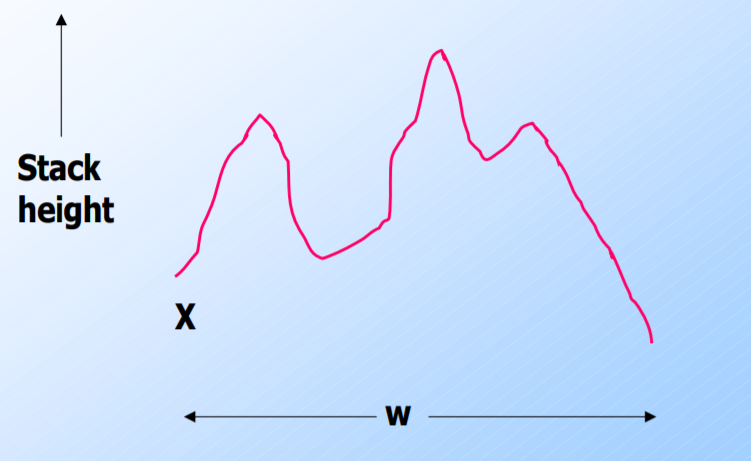
\includegraphics[scale=0.5]{popX.png}
        \caption{Plot showing popping of X}
        \label{fig:my_label}
    \end{figure}
    \end{center}
\begin{itemize}
    \item Now, assume L = N(P).
    \item We’ll construct a CFG G such that L = L(G).
    \item \textbf{Intuition:} G will have variables [pXq] generating exactly the inputs that cause P to have the net effect of popping stack symbol X while going from state p to state q.
    \item This variable generates all and only the strings w such that (p, w, X) $\vdash^*$ (q, $\epsilon$, $\epsilon$).
    \item P never gets below this X while doing so
    \item Each \textbf{production} for [pXq] comes from a move of P in state p with stack symbol X. 
\end{itemize}
\textbf{Productions of G can in general case be concluded as:}
\begin{itemize}
    \item Suppose $\delta$ (p, a, X) contains (r, Y$_1$,$\ldots$Y$_k$) for some state r and k $>$ 3.
    \item Generate family of productions [pXq] $\rightarrow$ a[rY$_1$s$_1$] [s$_1$Y$_2$s$_2$] $\ldots$ [s$_{k-2}$Y$_{k-1}$s$_{k-1}$][s$_{k-1}$Y$_{k}$q]
\end{itemize}
\subsubsection{Example:}
$\delta$ (p, a, X) contains (r, YZ) for some state r and symbols Y
and Z. Now, P has replaced X by YZ. To have the net effect of erasing X, P must erase Y, going from state r to some state s, and then erase Z, going from s to q. Hence, [pXq] $\rightarrow$ a[rYs][sZq]
\begin{figure}[h]
    \centering
    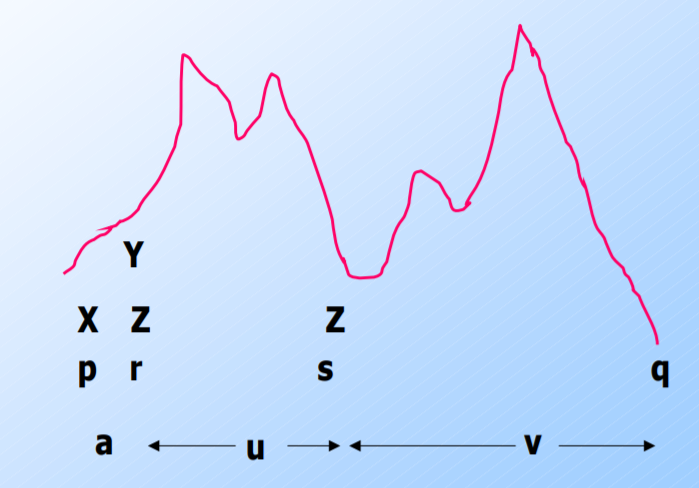
\includegraphics[scale=0.5]{popXYZ.png}
    \caption{Plot showing popping of XYZ}
    \label{fig:my_label}
\end{figure}
\section{The Pumping Lemma}
Simple intuition would be that we can always find two pieces of any sufficiently long string to “pump” in tandem. \textbf{That is:} if we repeat each of the two pieces the same number of times, we get another string in the language.
\begin{theorem}
For every context-free language L, there is an integer n, such that For every string z in L of length $\geqslant$ n. There exists z = uvwxy such that:
\begin{enumerate}
    \item $|$vwx$| \leqslant$ n
    \item $|$vx$| >$ 0
    \item For all i $\geqslant$ 0, uv$^i$wx$^i$y is in L;
\end{enumerate}
\end{theorem}
\subsection{Informal Proof:}
We will proof this by considering a CNF grammar with m varibles and take n = 2$^m$ and z be length greater or equal to n. Any parse tree which yield of z must have path of at least m+2 length or more (as in limiting case it'll resemble a binary tree which will have maximum of 2$^m$ children) From the previous statement it is clear that the parse tree will have at least m+1 variables and since our grammar has only m variables as stated in the beginning,  we can find two nodes with the same label, say A. \\
\par
V and x are the portions of the yield of the yellow tree that precede and
follow W respectively in the figure. Let u and y be the portions of z that precede v and follow x respectively. Let's look at the yellow. Since the path shown is as long as any other. And that path has at most m+1 variables. We know by the lemma 1 that we just proved, that the yield of the yellow plus purple is no longer than 2 to the power m, or n. \\ 
\begin{figure}[h]
    \centering
    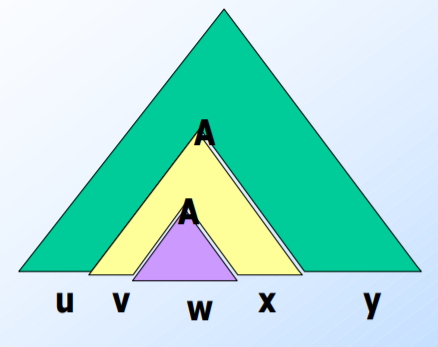
\includegraphics[scale=0.5]{pump1.png}
    \caption{Parse Tree (only the bottom branches)}
    \label{fig:my_label}
\end{figure}
\par
Moreover, once we have a variable automaton path there are no epsilon productions so
we must generate from this variable at least one terminal. That is all we need to conclude that either V or X or both have length at least one.\\
\begin{figure}[h]
    \centering
    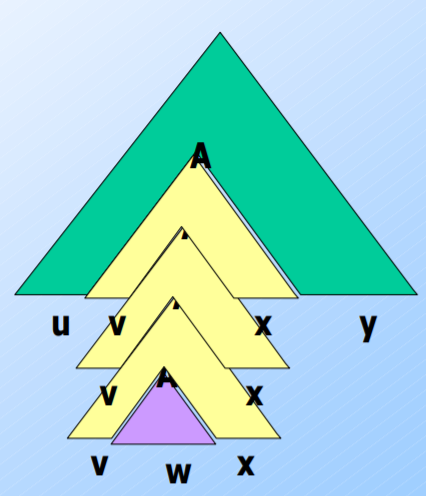
\includegraphics[scale=0.5]{pump3.png}
    \caption{Plot showing pumming thrice}
    \label{fig:my_label}
\end{figure} 
\textbf{Example:} We can prove that z = 0$^n$10$^n$10$^n$ is not a context-free language.


\chapter{Digital Circuits}
% \begin{itemize}
%     \item An analog signal $x(t)$ is represented by a real number at a given time point.
%     \item A digital signal is “binary” in nature, i.e., it takes on only two values: low (0) or high (1). 
%     \item Although we have shown 0 and 1 as constant levels, in reality, that is not required. Any value in the low (high) band will be interpreted as 0 (1) by digital circuits.
% \end{itemize}
\section{Logical Operations}
\begin{center}
\begin{tabular}{|c|c|c|c|}
 \hline
    Operation & Gate & Truth Table & Notation \\ \hline
     NOT & \begin{circuitikz} \draw
            (0,0) node[not port] (NOT) {};
                \end{circuitikz}  & \begin{tabular}{|c|c|}
                                        \hline
                                        \textbf{A} & \textbf{Y} \\ \hline 
                                        0 & 1 \\ \hline 
                                        1 & 0 \\ \hline 
                                        \end{tabular}
                                                    & $Y=\overline{A}$ \\ \hline
                                                                           \hline
     AND & \begin{circuitikz} \draw
            (0,0) node[and port] (AND) {};
                \end{circuitikz}  & 
                                   \begin{tabular}{|c|c|c|}
                                    \hline
                                   \textbf{A} & \textbf{B} & \textbf{Y} \\ \hline 
                                   0 & 0 & 0 \\ \hline 
                                   1 & 0 & 0 \\ \hline 
                                   0 & 1 & 0 \\ \hline
                                   1 & 1 & 1 \\ \hline
                                  \end{tabular}
                                                 & $Y=A.B$ \\ \hline \hline
     OR & \begin{circuitikz} \draw
            (0,0) node[or port] (OR) {};
                \end{circuitikz}  & 
                                    \begin{tabular}{|c|c|c|}
                                    \hline
                                   \textbf{A} & \textbf{B} & \textbf{Y} \\ \hline 
                                   0 & 0 & 0 \\ \hline 
                                   1 & 0 & 1 \\ \hline 
                                   0 & 1 & 1 \\ \hline
                                   1 & 1 & 1 \\ \hline
                                  \end{tabular}
                                                & $Y=A+B$ \\ \hline \hline
     NAND & \begin{circuitikz} \draw
            (0,0) node[nand port] (NAND) {};
                \end{circuitikz}  & \begin{tabular}{|c|c|c|}
                                    \hline
                                   \textbf{A} & \textbf{B} & \textbf{Y} \\ \hline 
                                   0 & 0 & 1 \\ \hline 
                                   1 & 0 & 1 \\ \hline 
                                   0 & 1 & 1 \\ \hline
                                   1 & 1 & 0 \\ \hline
                                  \end{tabular} 
                                                & $Y=\overline{A.B}$ \\ \hline \hline
     NOR & \begin{circuitikz} \draw
            (0,0) node[nor port] (NOR) {};
                \end{circuitikz}  & \begin{tabular}{|c|c|c|}
                                    \hline
                                   \textbf{A} & \textbf{B} & \textbf{Y} \\ \hline 
                                   0 & 0 & 1 \\ \hline 
                                   1 & 0 & 0 \\ \hline 
                                   0 & 1 & 0 \\ \hline
                                   1 & 1 & 0 \\ \hline
                                  \end{tabular}
                                               & $Y=\overline{A+B}$ \\ \hline \hline    
     XOR & \begin{circuitikz} \draw
            (0,0) node[xor port] (XOR) {};
                \end{circuitikz}  & \begin{tabular}{|c|c|c|}
                                    \hline
                                   \textbf{A} & \textbf{B} & \textbf{Y} \\ \hline 
                                   0 & 0 & 0 \\ \hline 
                                   1 & 0 & 1 \\ \hline 
                                   0 & 1 & 1 \\ \hline
                                   1 & 1 & 0 \\ \hline
                                  \end{tabular}
                                    & $Y=A\overline{B}+\overline{A}B$ \\ \hline \hline
                            
\end{tabular}
\end{center}
%https://www.kleemans.ch/diagrams-for-logic-in-latex
\subsection{Sum of Products (SOP)}
Sum of product form is a form of expression in Boolean algebra in which different product terms of inputs are being summed together. This product is not arithmetical multiply but it is Boolean logical AND and the Sum is Boolean logical OR.
\subsubsection{Example:}
X $=$ X$_1$ $+$ X$_2$ $+$ X$_3$ $+$ X$_4$ $=$ $\overline{A} B \overline{C} + \overline{A} BC + A \overline{BC} + AB \overline{C}$  
\begin{center}
\begin{tabular}{|c|c|c|c|c|c|c|c|}
 \hline
    A & B & C & X$_1$ & X$_2$ & X$_3$ & X$_4$ & X  \\ \hline
    0 & 0 & 0 & 0 & 0 & 0 & 0 & 0\\
    0 & 0 & 1 & 0 & 0 & 0 & 0 & 0\\
    0 & 1 & 0 & 1 & 0 & 0 & 0 & 1\\
    0 & 1 & 1 & 0 & 1 & 0 & 0 & 1\\
    1 & 0 & 0 & 0 & 0 & 1 & 0 & 1\\
    1 & 0 & 1 & 0 & 0 & 0 & 0 & 0\\
    1 & 1 & 0 & 0 & 0 & 0 & 1 & 1\\
    1 & 1 & 1 & 0 & 0 & 0 & 0 & 0\\
 \hline
\end{tabular}
\end{center}
This form is called the standard sum-of-products form, and each individual term (consisting of all three variables) is called a \textbf{“minterm"}.
\section{Product of sums (POS)}
The short form of the product of the sum is POS, and it is one kind of Boolean algebra expression. In this, it is a form in which products of the dissimilar sum of inputs are taken, which are not arithmetic result \& sum although they are logical Boolean AND \& OR correspondingly.
\subsubsection{Example:}
X = $(A + B + C) (\overline{A} + B + C) (\overline{A} + \overline{B} + C)$. \\
This form is called the standard product-of-sums form, and each individual term (consisting of all three variables) is called a \textbf{“maxterm.”}

\subsection{The X condition}
This is also called as \textbf{I don't care condition}. We'll understand this with the help of an example. I want to design a box (with inputs A, B, C, and output S) which will help in scheduling my appointments.
\begin{itemize}
    \item A $\rightarrow$ I am in town, and the time slot being suggested for the appointment is free.
    \item B $\rightarrow$ My favourite player is scheduled to play a match (which I can watch on TV).
    \item C $\rightarrow$ The appointment is crucial for my business.
    \item S $\rightarrow$ Schedule the appointment.
\end{itemize}
The following truth table summarizes the expected functioning of the box.
\begin{center}
\begin{tabular}{ |c|c|c|c| } 
 \hline
 A & B & C & S \\ \hline
 0 & X & X & 0 \\ 
 1 & 0 & X & 1 \\ 
 1 & 1 & 0 & 0 \\ 
 1 & 1 & 1 & 1 \\ 
 \hline
\end{tabular}
\end{center}
Note that we have a new entity called X in the truth table. X can be 0 or 1 (it does not matter) and is therefore called the “don’t care” condition. Don’t care conditions can often be used to get a more efficient implementation of a logical function.

\section{Karnaugh Maps}
A Karnaugh map (“K-map”) is a representation of the truth table of a logical
function. A K-map can be used to obtain a \textbf{“minimal” expression} of a function in the sum-of-products form or in the product-of-sums form. A “minimal” expression has a minimum number of terms, each with a minimum number of variables. (For some functions, it is possible to have more than one minimal expressions, i.e., more than one expressions with the same complexity.) It can be implemented with fewer gates.
\subsubsection{The 1’s can be enclosed by a rectangle in each case.}
\textbf{Minimal:} smallest number of terms, smallest number of variables in each term.\\
$\rightarrow$ smallest number of rectangles containing 2k 1’s, each as large as possible.
\subsubsection{Examples:}
We begin by explaining the smallest representation of a K-map. We mark the 1s by red and green color in the figure. It is a way to represent the NOR-Gate i.e. $\overline{A+B}$. 

\begin{center}
\begin{Karnaughquatre}
    \minterms{1,2}
    \maxterms{0,3}
     \implicantsol{1}{green}
     \implicantsol{2}{red}
\end{Karnaughquatre}
\end{center}

Now the example below is the representation of $BC \overline{A} + A \overline{BC}$. We have two "I don't care" situations and we mark them by assuming to be 1. 

\begin{center}
\begin{Karnaughvuit}
       \minterms{3,4}
        \maxterms{0,1,6,7}
       \indeterminats{2,5}
       \implicant{3}{2}{green}
       \implicant{4}{5}{orange}
    \end{Karnaughvuit}  
\end{center}
In this final example we rather mark all the 0's which are all here and different colors represent different ways in which they're marked. 
\begin{center}
\begin{Karnaugh}
        \contingut{0,0,0,0,0,0,0,0,0,0,0,0,0,0,0,0}
       \implicant{0}{2}{red}
       \implicant{5}{15}{purple}
       \implicantdaltbaix[3pt]{3}{10}{blue}
    \implicantcantons[2pt]{orange}
       \implicantcostats{4}{14}{green}
    \end{Karnaugh}
\end{center}

\section{Adder circuit}
\textbf{Adder circuit} is a combinational digital circuit that is used for adding two numbers. A typical adder circuit produces a sum bit (denoted by S) and a carry bit (denoted by C) as the output. Typically adders are realized  for adding binary numbers but they can be also realized  for adding other formats like BCD (binary coded decimal, XS-3 etc. Besides addition, adder circuits can be used for a lot of other applications in digital electronics like address decoding, table index calculation etc.

\subsection{Half Adder}
\textbf{Half adder} is a combinational  arithmetic circuit that adds two numbers and produces a sum bit (S) and carry bit (C) as the output. If  A and B are the input bits, then sum bit (S) is the X-OR of A and B  and the carry bit (C) will be the AND of A and B. From this it is clear that a half adder circuit can be easily constructed using one X-OR gate and one AND gate. Half adder is the simplest of all adder circuit, but it has a major disadvantage.  The half adder can add only two input bits (A and B) and has nothing to do with the carry if there is any in the input. So if the input to a half adder have a carry, then it will be neglected it and adds only the A and B bits. That means the binary addition process is not complete and that’s why it is called a half adder.
\subsubsection{Truth table of Half Adder}
\begin{center}
\begin{tabular}{ |c|c|c c| } 
 \hline
 A & B & C$_0$ & S \\ \hline
 0 & 0 & 0 & 0 \\ 
 1 & 0 & 0 & 1 \\ 
 0 & 1 & 0 & 1 \\ 
 1 & 1 & 1 & 0 \\ 
 \hline
\end{tabular}
\end{center}
\subsubsection{Circuit Diagrams}
\begin{figure}[h]
    \centering
    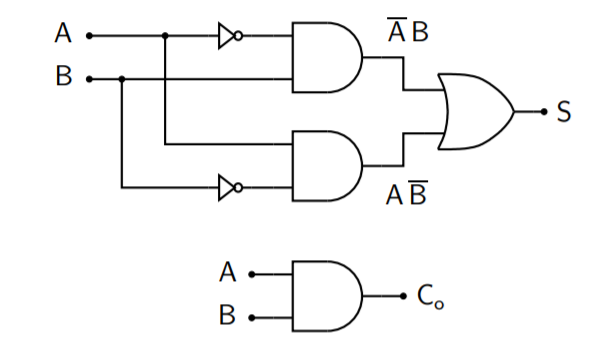
\includegraphics[scale=0.5]{impli1.png}
    \caption{Implementation 1}
    \label{fig:my_label}
\end{figure} 
\begin{figure}[h]
    \centering
    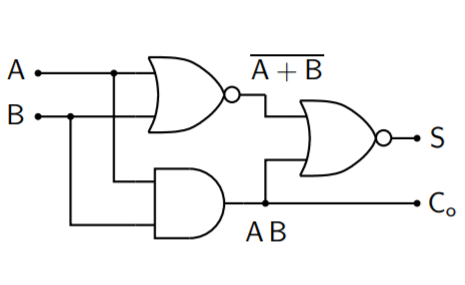
\includegraphics[scale=0.5]{impli2.png}
    \caption{Implementation 2}
    \label{fig:my_label}
\end{figure} 

\subsection{Full Adder}
Full Adder is the adder which adds three inputs and produces two outputs. The first two inputs are A and B and the third input is an input carry as C$_{in}$. The output carry is designated as C$_0$ and the normal output is designated as S which is SUM.
\subsubsection{Truth table}
\begin{center}
\begin{tabular}{|c|c|c|c|c|}
 \hline
    A & B & C$_{in}$ & C$_0$ & S  \\ \hline
    0 & 0 & 0 & 0 & 0 \\
    0 & 0 & 1 & 0 & 1 \\
    0 & 1 & 0 & 0 & 1 \\
    0 & 1 & 1 & 1 & 0 \\
    1 & 0 & 0 & 0 & 1 \\
    1 & 0 & 1 & 1 & 0 \\
    1 & 1 & 0 & 1 & 0 \\
    1 & 1 & 1 & 1 & 1 \\

 \hline
\end{tabular}
\end{center}

\section{Multiplexer}
The multiplexer, shortened to “MUX” or “MPX”, is a combinational logic circuit designed to switch one of several input lines through to a single common output line by the application of a control signal. Multiplexers operate like very fast acting multiple position rotary switches connecting or controlling multiple input lines called “channels” one at a time to the output.

\subsubsection{Truth Table}
\begin{center}
\begin{tabular}{ |c|c|c| } 
 \hline
 S$_1$ & S$_0$ & Z \\ \hline
 0 & 0 & I0 \\ 
 0 & 1 & I1 \\ 
 1 & 0 & I2 \\ 
 1 & 1 & I3 \\ 
 \hline
\end{tabular}
\end{center}
\subsubsection{Board Diagram}
On any input one of the I0-I3 get matched with the output Z.
\begin{figure}[h]
    \centering
    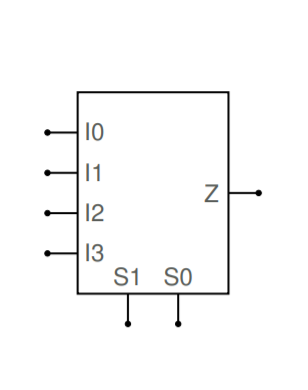
\includegraphics[scale=0.5]{mux_board.png}
    \caption{MUX Board Diagram}
    \label{fig:my_label}
\end{figure} 
\subsubsection{8-to-1 type MUX}
The board described in above example is a 4-to-1 type it can even be 8-to-1 type as shown in figure below. 
\begin{figure}[h]
    \centering
    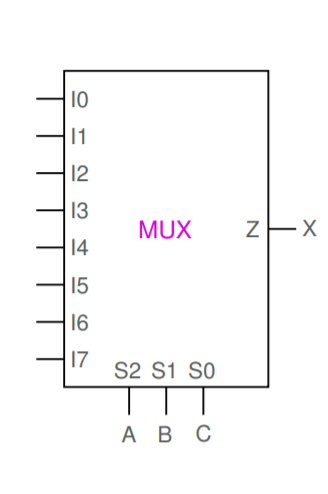
\includegraphics[scale=0.5]{8to1.png}
    \caption{8-to-1 MUX}
    \label{fig:my_label}
\end{figure} 
\newpage
\subsubsection{Circuit Diagram}
\begin{figure}[h]
    \centering
    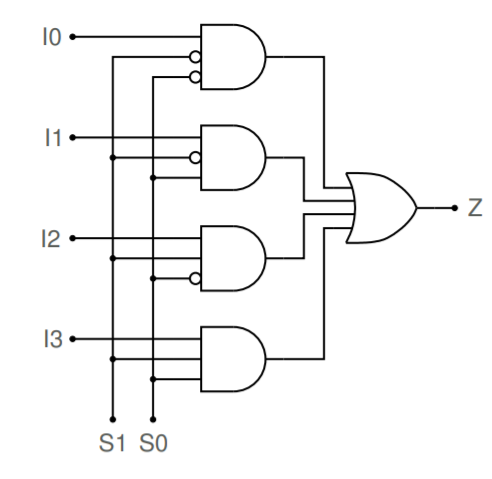
\includegraphics[scale=0.5]{mux_cir.png}
    \caption{MUX Circuit Diagram}
    \label{fig:my_label}
\end{figure} 
\textbf{The VHDL code for multiplexer is given in the next chapter.}
\newpage
\section{Decoders}
Decoder is a combinational circuit that has ‘n’ input lines and maximum of $2^n$ output lines. One of these outputs will be active High based on the combination of inputs present, when the decoder is enabled.
\subsubsection{Truth Table}
Below is the truth table image for 3-to-8 type decoder (didn't code because of more columns \& complicated structure).
\begin{figure}[h]
    \centering
    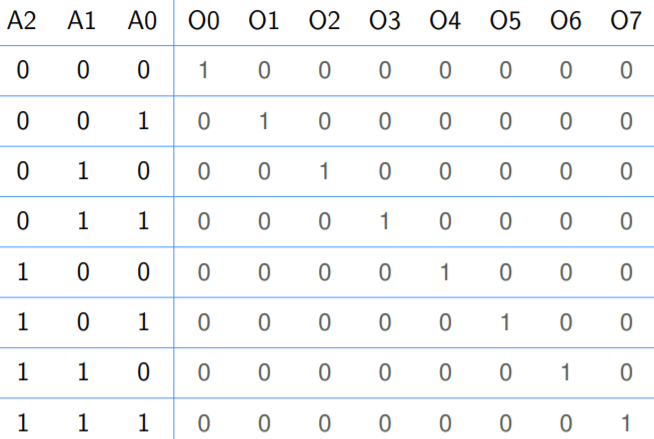
\includegraphics[scale=0.5]{dec_tt.png}
    \caption{Truth table}
    \label{fig:my_label}
\end{figure} 
\subsubsection{Board Diagram}
\begin{figure}[h]
    \centering
    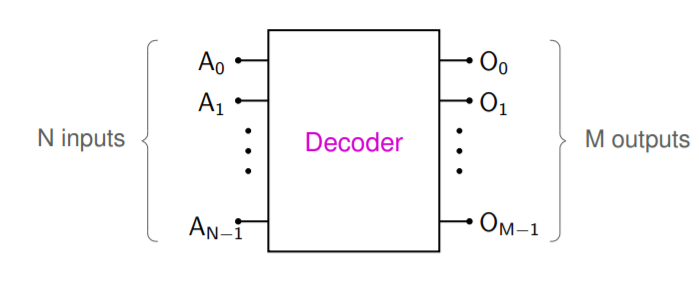
\includegraphics[scale=0.5]{enc_borad.png}
    \caption{Decoder Board Diagram}
    \label{fig:my_label}
\end{figure} 

%%FSM (doubtful)

\chapter{VHDL}
VHDL is a structured hardware description language for writing logic circuits. The V is short for yet another acronym: VHSIC or \textbf{Very High-Speed Integrated Circuit} and the HDL stands for \textbf{Hardware Description Language}. The nice thing about VHDL is that the level of detail is unambiguous due to the rich syntax rules associated with it. In other words, VHDL provides everything that is necessary in order to describe any digital circuit. Likewise, a digital circuit/system is any circuit that processes or stores digital information. Second, having some type of circuit model allows for the subsequent simulation and/or testing of the circuit. The VHDL model can also be translated into a form that can be used to generate actual working circuits. 
\section{Terminology}
\subsubsection{Stimulation}
\textit{Stimulation} is the prediction of the behaviour of a design:
\begin{itemize}
    \item VHDL provides many features suitable for the stimulation of digital design circuits.
    \item \textit{Functional stimulation} approximates the behaviour of a hardware design by assuming that all outputs change at the same time.
    \item \textit{Timing Stimulation} predicts the exact behaviour of a hardware design. 
\end{itemize}
\subsubsection{Synthesis}
\textit{Synthesis} is the transition of a design into a netlist file that describes the structure of a hardware description language.
\begin{itemize}
    \item VHDL was not designed for the purpose of synthesis.
    \item Not all VHDL statements are synthesizable. 
\end{itemize}
\subsubsection{FPGA}
A \textbf{Field Programmable Gate Array}, or FPGA, is a semiconductor device that comprises of logic blocks which are programmed to execute a specific set of functions. These programmable logic blocks are connected to each other with the help of an interconnect matrix.Hardware descriptive language key concepts, describing a hardware circuit implementation that your tool chain will eventually interpret and synthesize into FPGA logic cells. So whether it’s schematic based or hardware descriptive language based, the tool has the ability to synthesize this description into logic cells. 
\subsubsection{Invariants}
VHDL is not case sensitive and not even sensitive white spaces. Comments in VHDL begin with the symbol “$--$”. 
\section{Design Units}
\subsection{Entity}
The VHDL entity construct provides a method to abstract the functionality of a circuit description to a higher level. It provides a simple wrapper for the lower-level circuitry. This wrapper effectively describes how the black box interfaces with the outside world. Since VHDL describes digital circuits, the entity simply lists the various inputs and outputs of the underlying circuitry. In VHDL terms, the black box is described by an entity declaration.
\subsection{Standard Libraries}
The VHDL language as many other computer languages, has gone through a long and intense evolution. Among the most important standardization steps we can mention are the release of the IEEE Standard 1164 package as well as some child standards that further extended the functionality of the language. In order to take advantage of the main implementable feature of VHDL you just need to import the two main library packages i.e. IEEE.std\_logic\_1164.all and IEEE.numeric\_std.all. 
\subsection{Architecture}
The VHDL entity declaration, introduced before, describes the interface or the external representation of the circuit. The architecture describes what the circuit actually does. In other words, the VHDL architecture describes the internal implementation of the associated entity. As you can probably imagine, describing the external interface to a circuit is generally much easier than describing how the circuit is intended to operate. This statement becomes even more important as the circuits you are describing
become more complex. 
\subsection{Signals \& Variables}
In VHDL there are several object types. Among the most frequently used
we will mention the \textbf{signal} object type, the \textbf{variable} object type and the \textbf{constant} object type. The signal type is the software representation of a wire. The variable type, like in C or Java, is used to store local information. The constant is like a variable object type, the value of which cannot be changed.

\section{Programming Paradigm}
\subsubsection{Signal Assignment Operator $<=$}
Algorithmic programming languages always have some type of assignment
operator. In C or Java, this is the well-known “=” sign. In these languages, the assignment operator signifies a transfer of data from the right-hand side of the operator to the left-hand side. VHDL uses two consecutive characters to represent the assignment operator: “$<=$”. This combination was chosen because it is different from the assignment operators in most other common algorithmic programming languages. The operator is officially known as a \textbf{signal assignment operator} to highlight its true purpose.
\section{Logic Gates using VHDL}
This and further sections will contain the code VHDL code for designing digital circuits. I will not include all the codes here as it is present in the GitHub Repository\footnote{\href{https://github.com/Liza23/Summer-of-Science_Automata-Theory}{Automata Theory- Digital Circuits}}that I've created for this project.
\subsection{Or Gate}
In the example shown below I've tried to code the \textbf{or gate} with the inputs as x and y and output as z. 
\begin{minted}{vhdl}
library ieee;
use ieee.std_logic_1164.all;

entity or_gate is
port(x in std_logic;
     y in std_logic;
     z out std_logic
);
end or_gate;

architecture arch of or_gate is
begin
	process(x, y)
	begin
	if ((x='0') and (y='0')) then
		z <= '0';
	else 
		z <= '1';
	end if;
	end process;

end arch;

architecture beh of or_gate is
begin
	z <= x or y
end beh
\end{minted}
%image

\subsection{Xor Gate}
Here, in the example shown below I've tried to code the \textbf{xor gate} with the inputs as x and y and output as z. 

\begin{minted}{vhdl}
library ieee;
use ieee.std_logic_1164.all;

entity xor_gate is
port(x in std_logic;
     y in std_logic;
     z out std_logic
);
end xor_gate;

architecture arch of xor_gate is 
begin
	process(x, y)
	begin
	if (x/=y) then 
		z <='1';
	else 
		z <='0';
	end if;
	end process;
	
end arch;

architecture beh of xor_gate is 
begin 
	z <= x xor y;
end beh
\end{minted}
\subsubsection{Xor Gate Simulations}
\section{Multiplexer}
The functioning of a multiplexer is explained in the digital circuits sections here I've only tried to show it's basic code in testbench and design formats. It is a 4-to-1 MUX with inputs as I0, I1, I2, I3 and ouput as S. On any given input S becomes either of the inputs given. 
\subsubsection{Design}
\begin{minted}{vhdl}
library ieee;
use ieee.std_logic_1164.all;

entity multiplexer is
port( I3:   in std_logic_vector(2 downto 0)
      I2:   in std_logic_vector(2 downto 0)
      I1:   in std_logic_vector(2 downto 0)
      I0:   in std_logic_vector(2 downto 0)
      S:    in std_logic_vector(1 downto 0)
      O:    out std_logic_vector(2 downto 0)
);
end multiplexer;

architecture beh1 of multiplexer is
begin 
  process(I3,I2,I1,I0,S)
  begin
    case S is 
      when "00" =>    O <= I0;
      when "10" =>    O <= I1;
      when "01" =>    O <= I2;
      when "11" =>    O <= I3;
      when others =>  O <= "ZZZ";
    end case;
  
  end process;
end beh1;

architecture beh2 of multiplexer is
begin
  O <=    I0 when S = "00" else
          I1 when S = "01" else
          I2 when S = "10" else
          I3 when S = "11" else
          "ZZZ";
end beh2;
\end{minted}
\subsubsection{Testbench}
A test bench is VHDL code that allows you to provide a documented, repeatable set of stimuli that is portable across different simulators. A test bench can be as simple as a file with clock and input data or a more complicated file that includes error checking, file input and output, and conditional testing.

\begin{minted}{vhdl}
library IEEE;
use IEEE.std_logic_1164.all;
use IEEE.std_logic_arith.all;

entity multiplexer_tb is			
-- empty entity
end multiplexer_tb;

architecture testbench of multiplexer_tb is

    -- initialize the declared signals  
    signal T_I3: std_logic_vector(2 downto 0):="000"; 
    signal T_I2: std_logic_vector(2 downto 0):="000";
    signal T_I1: std_logic_vector(2 downto 0):="000";
    signal T_I0: std_logic_vector(2 downto 0):="000";
    signal T_O:  std_logic_vector(2 downto 0);
    signal T_S:  std_logic_vector(1 downto 0);
	
    component multiplexer_tb
    port( I3: 	in std_logic_vector(2 downto 0);
	  I2: 	in std_logic_vector(2 downto 0);
	  I1: 	in std_logic_vector(2 downto 0);
	  I0: 	in std_logic_vector(2 downto 0);
	  S:	  in std_logic_vector(1 downto 0);
	  O:	  out std_logic_vector(2 downto 0)
    );
    end component;

begin

    U_Mux: multiplexer port map (T_I3, T_I2, T_I1, T_I0, T_S, T_O);
	
    process							
	
	variable err_cnt: integer :=0;
	
    begin								
			 	
	T_I3 <= "001";		-- I0-I3 are different signals
	T_I2 <= "010";
	T_I1 <= "101";
	T_I0 <= "111";
		
	-- case select eqaul "00"
	wait for 10 ns;	
	T_S <= "00";	
	wait for 1 ns;
	assert (T_O="111") report "Error Case 0" severity error;
	if (T_O/="111") then 
	    err_cnt := err_cnt+1;
	end if;
		
	-- case select equal "01"
	wait for 10 ns;
	T_S <= "01";	  
	wait for 1 ns;
	assert (T_O="101") report "Error Case 1" severity error;
	if (T_O/="101") then 
	    err_cnt := err_cnt+1;
	end if;
		
	-- case select equal "10"
	wait for 10 ns;
	T_S <= "10";	  
	wait for 1 ns;
	assert (T_O="010") report "Error Case 2" severity error;
	if (T_O/="010") then 
	    err_cnt := err_cnt+1;
	end if;		
			
	-- case select equal "11"
	wait for 10 ns;
	T_S <= "11";	  
	wait for 1 ns;
	assert (T_O="001") report "Error Case 3" severity error;		
	if (T_O/="001") then 
	    err_cnt := err_cnt+1;
	end if;
			
	-- case equal "11"
	wait for 10 ns;
	T_S <= "UU";

	-- summary of all the tests
	if (err_cnt=0) then
	    assert (false) 
	    report "Testbench of Mux completed sucessfully!"
	    severity note;
	else
	    assert (true)
	    report "Something wrong, try again!"
	    severity error;
	end if;
		
	wait;
    
    end process;

end testbench;

configuration config of multiplexer_tb is
	for testbench
	end for;
end config;
\end{minted}

\section{Finite State Machines}
Finally, we code for sequential circuits and I'll include the code for its design and testbench both. A finite state machine (sometimes called a finite state automaton) is a computation model that can be implemented with hardware or software and can be used to simulate sequential logic and some computer programs. Finite state automata generate regular languages.

\subsubsection{Design}
\begin{minted}{vhdl}
library ieee;
use ieee.std_logic_1164.all;

entity seq_design is
port( a:      in std_logic;
      clock:  in std_logic;
      reset:  in std_logic;
      x:      out std_logic
);
end seq_design;

architecture fsm of seq_design is
  --design states of FSM model
  
  type state_type is (S0, S1, S2, S3);
  signal next_state, current_state: state_type;

begin
  --concurrent process#1: state registers
  state_reg: process(clock, reset)
  begin
    if (reset='1') then
      current_state <= S0;
    elif (clock'event and clock='1') then 
      current_state <= next_state;
    end if;
    
  end process;
  
  --concurrent process#2: combinational logic 
  comb_logic: process(current_state, a)
  
  begin
    --use case statement to show
    --state transition
    
    case current_state is
    
      when S0 => x <= '0';
               if a = '0' then 
                 next_state <= S0;
               elif a = '1' then
                 next_state <= S1;
               end if;
      
      when S1 => x<= '0';
               if a = '0' then
                 next_state <= S1;
               elif a = '1' then 
                 next_state <= S2;
               end if;
      
      when S2 => x <= '0';
               if a = '0' then 
                 next_state <= S2;
               elif a = '1' then
                 next_state <= S3;
               end if;
      
      when S3 => x<= '0';
               if a = '0' then
                 next_state <= S3;
               elif a = '1' then 
                 next_state <= S4;
               end if;
      
      when others =>
               x <= '0'
               next_state <= S0;
    
    end case;
    
  end process;

end fsm;   
\end{minted}

\subsubsection{Testbench}
A test bench is VHDL code that allows you to provide a documented, repeatable set of stimuli that is portable across different simulators. A test bench can be as simple as a file with clock and input data or a more complicated file that includes error checking, file input and output, and conditional testing.

\begin{minted}{vhdl}
library	ieee;
use ieee.std_logic_arith.all;  
use ieee.std_logic_unsigned.all;
use ieee.std_logic_1164.all;

entity fsm_tb is
--entity declaration
end fsm_tb;

architecture tb of fsm_tb is

signal T_a: std_logic;
signal T_clock: std_logic;
signal T_reset: srd_logic;
signal T_x: std_logic;

component seq_design
port( a:    in std_logic;
     clock: in std_logic;
     reset: in std_logic;
     x:     out std_logic
);
end component;
  
begin
  u_fsm: seq_design port map(T_a, T_clock, T_reset, T_x);
  
  process
  begin
    T_clock <= '1';
    wait for 5 ns;
    T_clock <= '0';
    wait for 5 ns;
  end process;
      
  process
      variable err_cnt: integer := 0;
  begin
    
    --case 1
    T_reset <= '1'
    wait for 20 ns;
    assert (T_x = '0') report "Failed Case 1" severity error;
    if (T_x/='0') then
      err_cnt := err_cnt+1;
    end if;
      
    --case 2
    T_reset <= '0'
    wait for 20 ns;
    assert (T_x = '0') report "Failed Case 2" severity error;
    if (T_x/='0') then
      err_cnt := err_cnt+1;
    end if;
    
    --case 3
    wait for 30 ns;
    T_a <= '1'
    wait for 35 ns;
    assert (T_x = '1') report "Failed Case 3" severity error;
    if (T_x/='1') then
      err_cnt := err_cnt+1;
    end if;
      
    --case 2
    wait for 70 ns;
    T_reset <= '1'
    wait for 10 ns;
    assert (T_x = '0') report "Failed Case 4" severity error;
    if (T_x/='0') then
      err_cnt := err_cnt+1;
    end if;
      
    --summary of all testcases
    if (err_cnt = 0) then 
      assert false
      report "Test bench executed succesfully!"
      severity note;
    
    else
      assert true
      report "Something is wrong!"
      severity note;
    end if;
      
    wait;
  
  end process;

end tb;
      
configuration cfg_tb of fsm_tb is
      for tb
      end for;
end cfg_tb;
\end{minted}
\subsubsection{\Large Conclusion}
This report not just contains various topics of automata theory but also has other different topics that revolve around the theory and which are essential for having a better understanding of the automata theory. It includes digital circuits and the code for some of those logic circuits and the link for the \href{https://github.com/Liza23/Summer-of-Science_Automata-Theory}{GitHub Repository} which contains code for all the logic circuits that I've studied as a part of the project.  
\end{document}
